\documentclass{article}%
\usepackage[T1]{fontenc}%
\usepackage[utf8]{inputenc}%
\usepackage{lmodern}%
\usepackage{textcomp}%
\usepackage{lastpage}%
%
\usepackage{amsmath}%
\usepackage{amssymb}%
\usepackage{amsfonts}%
\usepackage{graphicx}%
\usepackage{hyperref}%
\usepackage{tikz}%
\usepackage{pgfplots}%
\usetikzlibrary{math}%
\title{ITA 2026 - Química\thanks{This exam was solved and automatically generated with gpt-resolve: \url{https://github.com/lgabs/gpt-resolve}}}%
\author{claude{-}haiku{-}5{-}5 (solver) + claude{-}haiku{-}5{-}5 (judge)}%
\date{November 10, 2026}%
%
\begin{document}%
\normalsize%
\maketitle%
\section*{Questão 1}

\section*{Solução}

\textbf{Notação e hipóteses.} Sejam $c_1$, $c_2$ e $c_3$ as concentrações, em $\text{mol}\cdot\text{L}^{-1}$, do ácido na Solução 1, do ácido na Solução 2 e da base na Solução 3. O ácido monoprótico fraco é $\text{HA}$, com base conjugada $\text{A}^-$. A base monoprótica forte é $\text{MOH}$, totalmente dissociada em $\text{M}^+ + \text{OH}^-$. A "Solução I" do enunciado é a Solução 1. Adotamos $K_w = 1{,}0\times10^{-14}$ a 25~$^{\circ}$C, volumes aditivos e reação 1:1 entre ácido e base.

\textbf{Passo 1 (diluição).} Na diluição conserva-se a quantidade de matéria do soluto: $c_1 \cdot 4\ \text{mL} = c_2 \cdot 20\ \text{mL}$, logo
\[
c_1 = 5\,c_2 .
\]

\textbf{Passo 2 (estequiometria).} A neutralização é $\text{HA} + \text{OH}^- \rightarrow \text{A}^- + \text{H}_2\text{O}$, na proporção 1:1. No ponto de equivalência, $n(\text{HA}) = n(\text{OH}^-)$:
\[
c_2 \cdot 2\ \text{mL} = c_3 \cdot 38\ \text{mL} \quad\Rightarrow\quad c_3 = \frac{c_2}{19}.
\]

\textbf{Passo 3 (mistura no equivalente).} O volume final é $V = 2 + 38 = 40\ \text{mL}$. No equivalente não há excesso de ácido nem de base, e todo o ácido está como $\text{HA}$ ou $\text{A}^-$. Pelo balanço de massa, a concentração analítica $C$ de ácido na mistura é
\[
C = [\text{HA}] + [\text{A}^-] = \frac{c_2 \cdot 2\ \text{mL}}{40\ \text{mL}} = \frac{c_2}{20}.
\]

\textbf{Passo 4 (equilíbrio em pH = 12).} Com pH = 12, $[\text{H}^+] = 10^{-12}\ \text{mol}\cdot\text{L}^{-1}$ e
\[
[\text{OH}^-] = \frac{K_w}{[\text{H}^+]} = \frac{10^{-14}}{10^{-12}} = 10^{-2}\ \text{mol}\cdot\text{L}^{-1}.
\]

Balanço de cargas: $[\text{M}^+] + [\text{H}^+] = [\text{OH}^-] + [\text{A}^-]$. Balanço de massa do cátion: $[\text{M}^+] = C = [\text{HA}] + [\text{A}^-]$. Substituindo a segunda igualdade na primeira, obtemos a condição protônica:
\[
[\text{OH}^-] = [\text{HA}] + [\text{H}^+] \quad\Rightarrow\quad [\text{HA}] = 10^{-2} - 10^{-12} \approx 10^{-2}\ \text{mol}\cdot\text{L}^{-1},
\]
com erro relativo de $10^{-10}$, desprezível.

Pela constante do ácido, $K_A = [\text{H}^+][\text{A}^-]/[\text{HA}]$, logo
\[
\frac{[\text{A}^-]}{[\text{HA}]} = \frac{K_A}{[\text{H}^+]} = \frac{10^{-12}}{10^{-12}} = 1 \quad\Rightarrow\quad [\text{A}^-] = [\text{HA}].
\]
Isto decorre de $\text{pH} = \text{p}K_A = 12$. Portanto
\[
C = [\text{HA}] + [\text{A}^-] = 2\,[\text{HA}] \approx 2 \times 10^{-2}\ \text{mol}\cdot\text{L}^{-1}.
\]

Conferência pela hidrólise: $K_h = K_w/K_A = 10^{-2} = [\text{OH}^-][\text{HA}]/[\text{A}^-] = (10^{-2})(10^{-2})/(10^{-2})$, que confirma o resultado.

Observação: a fórmula simplificada $[\text{OH}^-] \approx \sqrt{K_h\,C}$ daria $C = 10^{-2}\ \text{mol}\cdot\text{L}^{-1}$ (e $c_2 = 0{,}20\ \text{mol}\cdot\text{L}^{-1}$). Ela só vale se a hidrólise for inferior a cerca de 5\%. Aqui a hidrólise atinge 50\%, por isso usamos o balanço completo.

\textbf{Passo 5 (resultados).}
\begin{itemize}
\item[a)] $c_2 = 20\,C = 20 \times 2 \times 10^{-2} = 0{,}40\ \text{mol}\cdot\text{L}^{-1}$.
\item[b)] $c_1 = 5\,c_2 = 5 \times 0{,}40 = 2{,}0\ \text{mol}\cdot\text{L}^{-1}$.
\item[c)] $c_3 = \dfrac{c_2}{19} = \dfrac{0{,}40}{19} = \dfrac{2}{95} \approx 2{,}1\times10^{-2}\ \text{mol}\cdot\text{L}^{-1}$.
\end{itemize}

\textbf{Verificações.}
\begin{itemize}
\item Quantidades de matéria: $n(\text{HA}) = 0{,}40 \times 2\times10^{-3} = 8{,}0\times10^{-4}$ mol e $n(\text{MOH}) = 2{,}1\times10^{-2} \times 38\times10^{-3} = 8{,}0\times10^{-4}$ mol, iguais como exige a equivalência.
\item Concentração final: $C = 8{,}0\times10^{-4}/0{,}040 = 2{,}0\times10^{-2}\ \text{mol}\cdot\text{L}^{-1}$. Com $[\text{OH}^-] = 10^{-2}$, tem-se pOH = 2 e pH = 12, como dado.
\item Ordem de grandeza: na Solução 2, $[\text{H}^+] \approx (K_A c_2)^{1/2} = (4\times10^{-13})^{1/2} \approx 6{,}3\times10^{-7}\ \text{mol}\cdot\text{L}^{-1}$, ionização da ordem de $10^{-6}$. Logo o ácido é de fato fraco, embora as aproximações de ácido fraco não tenham sido necessárias para o cálculo.
\end{itemize}

ANSWER: a) $c_2 = 0{,}40\ \text{mol}\cdot\text{L}^{-1}$; b) $c_1 = 2{,}0\ \text{mol}\cdot\text{L}^{-1}$; c) $c_3 = \dfrac{2}{95} \approx 2{,}1\times10^{-2}\ \text{mol}\cdot\text{L}^{-1}$%
\newpage%
\section*{Questão 2}

\section*{Solução}

\textbf{Hipóteses e convenções.}
\begin{itemize}
\item A reação é tratada como irreversível. O catalisador está em concentração constante e seu efeito fica todo em $k$: ele acelera a reação, mas não altera a estequiometria nem a quantidade final de O$_2$.
\item \textit{Convenção de velocidade:} $v=-\dfrac{d[\mathrm{H_2O_2}]}{dt}=k\,[\mathrm{H_2O_2}]$. A própria prova indica essa convenção. Com $v=-\tfrac{1}{2}\dfrac{d[\mathrm{H_2O_2}]}{dt}$, a constante efetiva seria $2k$ e a concentração em 5 min seria $0{,}5\cdot e^{-0{,}693}=0{,}25\ \mathrm{mol\cdot L^{-1}}$. A tabela, porém, traz $e^{-0{,}3465}$, que é exatamente $e^{-kt}$ com $kt=0{,}0693\cdot 5=0{,}3465$.
\item \textit{Volume constante:} $V=0{,}100\ \mathrm{L}$. A água formada (no máximo $0{,}050$ mol, cerca de $0{,}9$ mL) altera o volume em cerca de $1\,\%$, dentro da precisão dos dados.
\item \textit{Gás:} o O$_2$ formado é puro e sai da solução como gás ideal. Não há correção de pressão de vapor da água, pois a prova não fornece esse dado. A solubilidade do O$_2$ em água é desprezada, pelo mesmo motivo.
\end{itemize}

Quantidade inicial de H$_2$O$_2$:
\[
n_0=[\mathrm{H_2O_2}]_0\,V=0{,}5\ \mathrm{mol\cdot L^{-1}}\cdot 0{,}100\ \mathrm{L}=0{,}050\ \mathrm{mol}
\]

\textbf{1. Ordem da reação.} O coeficiente $2$ da equação não define a ordem, que é determinada experimentalmente. Admitindo lei de potência $v=k\,[\mathrm{H_2O_2}]^{n}$, sem dependência de O$_2$ e com catalisador em concentração fixa, a unidade de $k$ é $(\mathrm{mol\cdot L^{-1}})^{1-n}\cdot\mathrm{min^{-1}}$, pois $v$ está em $\mathrm{mol\cdot L^{-1}\cdot min^{-1}}$. Como $k$ é dada em $\mathrm{min^{-1}}$, tem-se $n=1$. A ordem zero exigiria $k$ em $\mathrm{mol\cdot L^{-1}\cdot min^{-1}}$, e a ordem dois, em $\mathrm{L\cdot mol^{-1}\cdot min^{-1}}$. Ambas são incompatíveis com o dado.

\textbf{2. Lei integrada.} Com $[\mathrm{A}]=[\mathrm{H_2O_2}]$ e $-\dfrac{d[\mathrm{A}]}{dt}=k\,[\mathrm{A}]$, separam-se as variáveis e integra-se de $t=0$ ($[\mathrm{A}]_0$) até $t$ ($[\mathrm{A}]$):
\begin{align*}
\int_{[\mathrm{A}]_0}^{[\mathrm{A}]}\frac{d[\mathrm{A}]}{[\mathrm{A}]}&=-k\int_0^{t}dt\\
\ln\frac{[\mathrm{A}]}{[\mathrm{A}]_0}&=-kt\\
[\mathrm{A}]&=[\mathrm{A}]_0\,e^{-kt}
\end{align*}
Para $t=0$ recupera-se $[\mathrm{A}]_0$. A exponencial decresce, como exige $d[\mathrm{A}]/dt<0$ com $k>0$. A meia-vida dá outra checagem:
\[
t_{1/2}=\frac{\ln 2}{k}=\frac{0{,}693}{0{,}0693}\ \mathrm{min}=10\ \mathrm{min}
\]
Em $t_{1/2}$, $[\mathrm{A}]=0{,}25\ \mathrm{mol\cdot L^{-1}}$, a metade da concentração inicial.

\textbf{a) Volume de O$_2$ ao término da reação.} Pela estequiometria, 2 mol de H$_2$O$_2$ produzem 1 mol de O$_2$, logo
\[
n_{\mathrm{O_2}}=\frac{n_0-n_{\mathrm{H_2O_2}}(t)}{2}
\]
Pela lei exponencial, $[\mathrm{A}]\to 0$ somente para $t\to\infty$. Toma-se como término o consumo praticamente total: em $t=100$ min ($10$ meias-vidas) resta $2^{-10}\approx 0{,}1\,\%$ do reagente, erro inferior à precisão dos dados. Assim,
\[
n_{\mathrm{O_2}}=\frac{0{,}050}{2}\ \mathrm{mol}=0{,}025\ \mathrm{mol}
\]
Esse valor não depende de $k$, pois o catalisador altera apenas o tempo necessário.

Gás ideal, com $T=25+273=298$ K e $P=1$ atm:
\[
V=\frac{n_{\mathrm{O_2}}\,R\,T}{P}=\frac{0{,}025\cdot 8{,}21\times10^{-2}\cdot 298}{1}\ \mathrm{L}\approx 0{,}612\ \mathrm{L}\approx 612\ \mathrm{mL}
\]
Unidades: $\mathrm{mol\cdot(atm\cdot L\cdot K^{-1}\cdot mol^{-1})\cdot K/atm=L}$.

Conferências: em CNTP, $0{,}025\cdot 22{,}4=0{,}56$ L; corrigido para 298 K, $0{,}56\cdot 298/273\approx 0{,}61$ L. Com $R=8{,}31$ J$\cdot$K$^{-1}\cdot$mol$^{-1}$ e $1$ atm $=1{,}01325\times10^{5}$ N$\cdot$m$^{-2}$, obtém-se $0{,}611$ L, com diferença de $0{,}1\,\%$ devida ao arredondamento de $R$.

\textbf{b) Concentração de H$_2$O$_2$ em 5 min.} O produto $kt=0{,}0693\ \mathrm{min^{-1}}\cdot 5\ \mathrm{min}=0{,}3465$ é adimensional, pois o minuto se cancela. Logo
\[
[\mathrm{H_2O_2}]=0{,}5\cdot e^{-0{,}3465}\ \mathrm{mol\cdot L^{-1}}=0{,}5\cdot 0{,}707\ \mathrm{mol\cdot L^{-1}}\approx 0{,}354\ \mathrm{mol\cdot L^{-1}}
\]
Conferências: $0{,}3465=\tfrac{1}{2}\ln 2$, pois $5$ min é metade de $t_{1/2}$. Logo $e^{-0{,}3465}=2^{-1/2}=1/\sqrt{2}\approx 0{,}707$, valor coincidente com o da tabela. O resultado está entre $0{,}5$ (em $t=0$) e $0{,}25$ (em $t_{1/2}$). Restam cerca de $71\,\%$ do reagente, com consumo de $0{,}146\ \mathrm{mol\cdot L^{-1}}$, menos da metade, como esperado para $t<t_{1/2}$.

ANSWER: a) $V(\mathrm{O_2})\approx 0{,}612\ \mathrm{L}$ (cerca de 612 mL, correspondente a $0{,}025$ mol de O$_2$ a $25\,^{\circ}\mathrm{C}$ e 1 atm); b) $[\mathrm{H_2O_2}]\approx 0{,}354\ \mathrm{mol\cdot L^{-1}}$ após 5 min.%
\newpage%
\section*{Questão 3}

\section*{Solução}

\textbf{Hipóteses e convenções.}
\begin{itemize}
\item Só a água vaporiza: A$^+$ e B$^-$ não são voláteis e permanecem na solução. Pela consideração iv, toda a potência $P$ é usada na vaporização da água. A solução já está a $100\,^\circ\text{C}$, portanto não há aquecimento sensível.
\item Consideração ii: a ebulição ocorre a 1 bar, e o enunciado fornece $\Delta H_{\text{ebulição}}$ da água nessa condição. A diferença para 1 atm ($1{,}01325$ bar) é desprezível frente à precisão dos dados (dois ou três algarismos significativos), por isso o valor fornecido é usado diretamente. Pelo mesmo motivo, a temperatura de ebulição é fixada em $100\,^\circ\text{C}$, desprezando-se a diferença real de cerca de $0{,}4\,^\circ\text{C}$ entre 1 bar e 1 atm.
\item Consideração iii: sem elevação ebulioscópica, a ebulição se mantém a $100\,^\circ\text{C}$ durante todo o processo.
\item Consideração i: o volume da solução é o volume do líquido, ou seja, o volume de água. Hipótese adicional, não explícita no enunciado: o sólido AB(s) é fase separada e seu volume é desprezado, pois a quantidade de sólido é da ordem de $10^{-3}$ mol.
\item Sem supersaturação: o sólido aparece exatamente quando $Q = K_{\text{PS}}$, com $Q = [\text{A}^+][\text{B}^-]$. A partir daí, enquanto houver AB(s) (fase pura, atividade unitária), a solução permanece saturada: $K_{\text{PS}} = [\text{A}^+][\text{B}^-]$.
\item Convenção do enunciado (atividades unitárias, efeitos não ideais desprezados): a atividade de cada íon é numericamente igual à sua concentração em $\text{mol}\cdot\text{L}^{-1}$. Na realidade $\gamma < 1$, mas o enunciado manda desprezar esse efeito.
\item Densidade $\rho = 1\ \text{g}\cdot\text{mL}^{-1}$, usada para converter massa de água evaporada em volume.
\end{itemize}

\textbf{Convenção numérica.} Os resultados são escritos com radicais exatos e avaliados com $\sqrt{3} \approx 1{,}732$ e $\sqrt{5} \approx 2{,}236$. Com os valores fornecidos no enunciado ($\sqrt{3} = 1{,}73$ e $\sqrt{5} = 2{,}24$), as diferenças aparecem apenas na terceira casa decimal, e os resultados com dois algarismos significativos são os mesmos.

\textbf{1. Vazão de evaporação (balanço de energia).} Em $t$ segundos, a energia fornecida é $P\,t$, que vaporiza a massa $m = \rho\,\Delta V$ de água:
\[
P\,t = m\,\Delta H_{\text{vap}} \;\Rightarrow\; \Delta V(t) = \frac{P\,t}{\rho\,\Delta H_{\text{vap}}} = \frac{540\ \text{cal}\cdot\text{s}^{-1}\times t}{1\ \text{g}\cdot\text{mL}^{-1}\times 540\ \text{cal}\cdot\text{g}^{-1}} = 1\ \text{mL}\cdot\text{s}^{-1}\times t
\]
(unidades: $\text{cal}\cdot\text{s}^{-1}\cdot\text{s}/(\text{g}\cdot\text{mL}^{-1}\cdot\text{cal}\cdot\text{g}^{-1}) = \text{mL}$). Portanto $V(t) = \left(1 - 1\times10^{-3}\,t\right)\ \text{L}$, com $t$ em segundos.

\textbf{2. Início da precipitação.} Enquanto não há sólido, as quantidades de matéria são fixas ($n_{\text{A}^+} = 2\times10^{-3}$ mol e $n_{\text{B}^-} = 1\times10^{-3}$ mol), e só a concentração varia com $V$:
\[
Q(V) = [\text{A}^+][\text{B}^-] = \frac{2\times10^{-3}}{V}\cdot\frac{1\times10^{-3}}{V} = \frac{2\times10^{-6}}{V^2}
\]
Em $V = 1$ L, $Q = 2\times10^{-6} < K_{\text{PS}} = 1\times10^{-5}$, logo ainda não há precipitado. O início ocorre quando $Q = K_{\text{PS}}$, no volume $V_p$:
\[
\frac{2\times10^{-6}}{V_p^2} = 1\times10^{-5} \;\Rightarrow\; V_p^2 = 0{,}2\ \text{L}^2 \;\Rightarrow\; V_p = \sqrt{0{,}2}\ \text{L} = \frac{\sqrt{5}}{5}\ \text{L} \approx \frac{2{,}236}{5}\ \text{L} = 0{,}4472\ \text{L}
\]

\textbf{Item a.} O volume de água evaporado até o início da precipitação é
\[
\Delta V = V(0) - V_p = (1 - 0{,}4472)\ \text{L} = 0{,}5528\ \text{L} = 552{,}8\ \text{mL}
\]
Rastro energético: a massa evaporada é $m = \rho\,\Delta V = 1\ \text{g}\cdot\text{mL}^{-1}\times 552{,}8\ \text{mL} = 552{,}8\ \text{g}$. O calor necessário é $q = m\,\Delta H_{\text{vap}} = 552{,}8\ \text{g}\times 540\ \text{cal}\cdot\text{g}^{-1} \approx 2{,}985\times10^{5}\ \text{cal}$, e o tempo é
\[
t = \frac{q}{P} = \frac{2{,}985\times10^{5}\ \text{cal}}{540\ \text{cal}\cdot\text{s}^{-1}} = 552{,}8\ \text{s} \approx 5{,}5\times10^{2}\ \text{s}
\]
Com $\sqrt{5} = 2{,}24$ o mesmo cálculo dá $V_p = 0{,}448$ L e $t = 552$ s. A diferença é só de arredondamento.

\textbf{Item b.} O volume pedido é
\[
V_f = \frac{V_p}{2} = \frac{\sqrt{5}}{10}\ \text{L} \approx 0{,}2236\ \text{L}, \qquad V_f^2 = \frac{V_p^2}{4} = 0{,}05\ \text{L}^2 \ \text{(exato)}
\]
Como $V_f < V_p$, já há AB(s) e a solução está saturada. Seja $x$ a quantidade de matéria de AB formada desde o início. Pela estequiometria 1:1:1,
\[
n_{\text{A}^+} = (2\times10^{-3} - x)\ \text{mol}, \qquad n_{\text{B}^-} = (1\times10^{-3} - x)\ \text{mol}, \qquad 0 \le x \le 1\times10^{-3}\ \text{mol}
\]
O limite superior vem de B$^-$ ser o reagente limitante, pois $n_{\text{B}^-} \ge 0$. A condição de saturação em $V_f$ é
\[
\frac{(2\times10^{-3} - x)(1\times10^{-3} - x)}{V_f^2} = 1\times10^{-5} \;\Rightarrow\; (2\times10^{-3} - x)(1\times10^{-3} - x) = 5\times10^{-7}\ \text{mol}^2
\]
Fazendo $x = y\times10^{-3}$ mol, com $y$ adimensional, e dividindo por $10^{-6}\ \text{mol}^2$:
\[
(2 - y)(1 - y) = 0{,}5 \;\Rightarrow\; y^2 - 3y + 1{,}5 = 0
\]
O discriminante é $\Delta = 9 - 6 = 3$, logo $y = \dfrac{3 \pm \sqrt{3}}{2}$, ou seja, $y_1 \approx 0{,}634$ e $y_2 \approx 2{,}366$. A raiz $y_2$ daria $n_{\text{B}^-} = (1 - 2{,}366)\times10^{-3}$ mol $< 0$, o que é impossível, e é descartada. Assim $y = \dfrac{3 - \sqrt{3}}{2} \approx 0{,}634$, isto é, $x \approx 0{,}634\times10^{-3}$ mol $< 1\times10^{-3}$ mol, compatível com o limite. Então
\[
n_{\text{A}^+} = \frac{1 + \sqrt{3}}{2}\times10^{-3}\ \text{mol} \approx 1{,}366\times10^{-3}\ \text{mol}, \qquad n_{\text{B}^-} = \frac{\sqrt{3} - 1}{2}\times10^{-3}\ \text{mol} \approx 0{,}366\times10^{-3}\ \text{mol}
\]
Dividindo pelo volume $V_f = \dfrac{\sqrt{5}}{10}$ L:
\[
[\text{A}^+] = \frac{(1+\sqrt{3})/2\times10^{-3}}{\sqrt{5}/10}\ \text{mol}\cdot\text{L}^{-1} = \sqrt{5}\,(1+\sqrt{3})\times10^{-3}\ \text{mol}\cdot\text{L}^{-1} \approx 6{,}11\times10^{-3}\ \text{mol}\cdot\text{L}^{-1}
\]
\[
[\text{B}^-] = \sqrt{5}\,(\sqrt{3}-1)\times10^{-3}\ \text{mol}\cdot\text{L}^{-1} \approx 1{,}64\times10^{-3}\ \text{mol}\cdot\text{L}^{-1}
\]
Com dois algarismos significativos, $[\text{A}^+] \approx 6{,}1\times10^{-3}$ e $[\text{B}^-] \approx 1{,}6\times10^{-3}$ mol$\cdot$L$^{-1}$.

\textbf{Verificações.}
\begin{itemize}
\item Produto de solubilidade: $[\text{A}^+][\text{B}^-] = \left(\sqrt{5}\right)^{2}(1+\sqrt{3})(\sqrt{3}-1)\times10^{-6} = 5\cdot 2\times10^{-6} = 1\times10^{-5} = K_{\text{PS}}$.
\item Continuidade: com $x = 0$, a equação de saturação fornece $V^2 = 0{,}2\ \text{L}^2$, ou seja, o próprio $V_p$.
\item Balanço de massa: $n_{\text{A}^+} + x = 2\times10^{-3}$ mol e $n_{\text{B}^-} + x = 1\times10^{-3}$ mol, com quantidades remanescentes positivas.
\item Sentido físico: sem precipitação, $[\text{A}^+] = 2\times10^{-3}/0{,}2236 \approx 8{,}9\times10^{-3}$ mol$\cdot$L$^{-1}$. O sólido retira $0{,}634$ mmol de A$^+$, e a concentração cai para $6{,}1\times10^{-3}$. Analogamente, $[\text{B}^-]$ cairia de $4{,}5\times10^{-3}$ para $1{,}6\times10^{-3}$ mol$\cdot$L$^{-1}$.
\item Unidades: $K_{\text{PS}}V_f^2$ tem unidade de mol$^2$, coerente com o lado esquerdo; as concentrações saem em mol$\cdot$L$^{-1}$; $t$ sai em segundos.
\item Ordem de grandeza: as concentrações são da ordem de $10^{-3}$ mol$\cdot$L$^{-1}$, com $[\text{A}^+] > [\text{B}^-]$, como esperado pelo excesso de A$^+$.
\end{itemize}

ANSWER: a) $t \approx 5{,}5\times10^{2}\ \text{s}$ (552,8 s; 552 s com $\sqrt{5} = 2{,}24$); b) $[\text{A}^+] \approx 6{,}1\times10^{-3}\ \text{mol}\cdot\text{L}^{-1}$ e $[\text{B}^-] \approx 1{,}6\times10^{-3}\ \text{mol}\cdot\text{L}^{-1}$%
\newpage%
\section*{Questão 4}

\section*{Solução}

\textbf{Hipóteses.}
\begin{itemize}
\item[(i)] Rendimento de 100\%: não há perda de Nb no preparo do BGN nem na termogravimetria; todo o Nb do sal está no BGN e no resíduo.
\item[(ii)] A amostra de oxalato é pura, a decomposição térmica é completa e o resíduo é exclusivamente $\mathrm{Nb_2O_5}$ (dado do enunciado).
\item[(iii)] A massa de referência da termogravimetria é a massa inicial do sal hidratado (inclui a água). Logo $m_{\mathrm{Nb_2O_5}} = 0{,}285\,m_{\text{sal}}$.
\item[(iv)] A composição molar refere-se às unidades de óxido: base de 100 mol de unidades-fórmula, com 60 mol de $\mathrm{SiO_2}$, 36 mol de $\mathrm{CaO}$ e 4 mol de $\mathrm{Nb_2O_5}$.
\end{itemize}

\textbf{Massas molares} (não fornecidas diretamente; calculadas com a tabela):
\[
M(\mathrm{SiO_2}) = 28{,}09 + 2\cdot 16{,}00 = 60{,}09\ \mathrm{g\,mol^{-1}},\qquad M(\mathrm{CaO}) = 40{,}08 + 16{,}00 = 56{,}08\ \mathrm{g\,mol^{-1}}
\]
\[
M(\mathrm{Nb_2O_5}) = 2\cdot 92{,}91 + 5\cdot 16{,}00 = 265{,}82\ \mathrm{g\,mol^{-1}}
\]

\textbf{Item a)}

\emph{Passo 1: fração mássica de $\mathrm{Nb_2O_5}$.} Porcentagem molar não é porcentagem mássica. Em 100 mol de unidades-fórmula:
\[
m_{\mathrm{BGN}} = 60\cdot 60{,}09 + 36\cdot 56{,}08 + 4\cdot 265{,}82 = 3605{,}40 + 2018{,}88 + 1063{,}28 = 6687{,}56\ \mathrm{g}
\]
\[
w(\mathrm{Nb_2O_5}) = \frac{1063{,}28}{6687{,}56} = 0{,}15899
\]
Os 4 mol de $\mathrm{Nb_2O_5}$ correspondem a 15,9\% em massa, porque a unidade $\mathrm{Nb_2O_5}$ é muito mais pesada que as de $\mathrm{SiO_2}$ e $\mathrm{CaO}$.

\emph{Passo 2: $\mathrm{Nb_2O_5}$ em 10 g de BGN.}
\[
m_{\mathrm{Nb_2O_5}} = 10\ \mathrm{g}\cdot 0{,}15899 = 1{,}5899\ \mathrm{g}
\]

\emph{Passo 3: massa de sal.} Pela hipótese (iii):
\[
m_{\text{sal}} = \frac{m_{\mathrm{Nb_2O_5}}}{0{,}285} = \frac{1{,}5899\ \mathrm{g}}{0{,}285} = 5{,}58\ \mathrm{g}
\]
Este passo não depende de $n$, pois a razão de 28,5\% já relaciona o resíduo à massa do sal hidratado. Como o dado tem três algarismos significativos, adota-se 5,58 g (cerca de 5,6 g). Pela hipótese (i), qualquer perda de Nb exigiria mais sal; portanto 5,58 g é um limite inferior.

\textbf{Item b)}

\emph{Passo 1: balanço de Nb.} Cada fórmula do sal contém 1 átomo de Nb e cada $\mathrm{Nb_2O_5}$ contém 2. Logo, pela hipótese (i), 1 mol de sal fornece $\tfrac{1}{2}$ mol de $\mathrm{Nb_2O_5}$. Essa relação basta para o cálculo: os gases liberados não entram nele. Uma equação ilustrativa em atmosfera oxidante (hipótese adicional, não usada no cálculo) é
\[
4\,\mathrm{NH_4[NbO(C_2O_4)_2]}\cdot n\,\mathrm{H_2O} + 7\,\mathrm{O_2} \longrightarrow 2\,\mathrm{Nb_2O_5} + 2\,\mathrm{N_2} + 16\,\mathrm{CO_2} + (8+4n)\,\mathrm{H_2O}
\]
Conferência por elemento: N: $4 = 2\cdot 2$; C: $16 = 16$; Nb: $4 = 2\cdot 2$; H: $4(4+2n) = 2(8+4n)$; O: $4(9+n)+14 = 2\cdot 5+16\cdot 2+(8+4n)$, ou seja, $50+4n = 50+4n$. Redox: N passa de $-3$ a $0$ (12 e$^-$ cedidos), C de $+3$ a $+4$ (16 e$^-$ cedidos), e os 7 $\mathrm{O_2}$ recebem 28 e$^-$. O Nb permanece em $+5$.

\emph{Passo 2: relação massa--massa.} Como $n_{\mathrm{Nb_2O_5}} = \tfrac{1}{2}\,n_{\text{sal}}$ e a razão do resíduo é 0,285:
\[
\frac{m_{\mathrm{Nb_2O_5}}}{m_{\text{sal}}} = \frac{M(\mathrm{Nb_2O_5})}{2\,M_{\text{sal}}} = 0{,}285
\quad\Rightarrow\quad
M_{\text{sal}} = \frac{265{,}82}{2\cdot 0{,}285} = 466{,}35\ \mathrm{g\,mol^{-1}}
\]

\emph{Passo 3: massa molar do sal anidro.}
\[
M(\mathrm{NH_4}) = 14{,}01 + 4\cdot 1{,}01 = 18{,}05;\quad M(\mathrm{NbO}) = 92{,}91 + 16{,}00 = 108{,}91;\quad M(\mathrm{C_2O_4}) = 2\cdot 12{,}01 + 4\cdot 16{,}00 = 88{,}02\ \mathrm{g\,mol^{-1}}
\]
\[
M_{\text{anidro}} = 18{,}05 + 108{,}91 + 2\cdot 88{,}02 = 303{,}00\ \mathrm{g\,mol^{-1}}
\]

\emph{Passo 4: água de hidratação.} Como $M_{\text{sal}} = M_{\text{anidro}} + n\,M(\mathrm{H_2O})$, com $M(\mathrm{H_2O}) = 2\cdot 1{,}01 + 16{,}00 = 18{,}02\ \mathrm{g\,mol^{-1}}$:
\[
n = \frac{466{,}35 - 303{,}00}{18{,}02} = \frac{163{,}35}{18{,}02} \approx 9{,}06
\]
Como $n$ é inteiro, $n = 9$.

\emph{Verificação.} Resíduo previsto $M(\mathrm{Nb_2O_5})/(2M_{\text{sal}})$ para os inteiros vizinhos:
\begin{itemize}
\item $n=8$: $M = 447{,}16\ \mathrm{g\,mol^{-1}}$, resíduo 29,72\% (desvio de 1,2 p.p.);
\item $n=9$: $M = 465{,}18\ \mathrm{g\,mol^{-1}}$, resíduo 28,57\% (desvio de 0,07 p.p.);
\item $n=10$: $M = 483{,}20\ \mathrm{g\,mol^{-1}}$, resíduo 27,51\% (desvio de 1,0 p.p.).
\end{itemize}
O valor 28,57\% arredondaria para 28,6\%; o 28,5\% do enunciado é compatível com truncamento ou com a precisão da leitura termogravimétrica. Nenhum outro inteiro se aproxima. Caso particular: usar a massa anidra (303,00 g/mol) daria resíduo de 43,9\%, incompatível com o dado. Isso confirma que a base da termogravimetria é o sal hidratado (hipótese iii).

\emph{Confirmação cruzada do item a).} Agora, com $M_{\text{sal}} = 465{,}18\ \mathrm{g\,mol^{-1}}$ ($n=9$):
\[
n_{\mathrm{Nb}} = 2\cdot\frac{1{,}5899}{265{,}82} = 1{,}1963\times 10^{-2}\ \mathrm{mol}
\qquad\Rightarrow\qquad
m_{\text{sal}} = 1{,}1963\times 10^{-2}\cdot 465{,}18 = 5{,}56\ \mathrm{g}
\]
A diferença para 5,58 g é de 0,014 g, isto é, 0,25\%. Ela é a razão $0{,}2857/0{,}285 \approx 1{,}0025$ entre o resíduo teórico e o dado. Vem do arredondamento 28,5\% frente a 28,57\%, e não de erro de cálculo. Ambos os resultados dão cerca de 5,6 g.

\textbf{Resposta.} a) $m_{\text{sal}} \approx 5{,}58\ \mathrm{g}$ (cerca de 5,6 g; limite inferior, ver hipótese (i)); b) $n = 9$, isto é, $\mathrm{NH_4[NbO(C_2O_4)_2]\cdot 9\,H_2O}$, com $M \approx 465\ \mathrm{g\,mol^{-1}}$.

ANSWER: a) $5{,}58\ \mathrm{g}$ (cerca de 5,6 g) de $\mathrm{NH_4[NbO(C_2O_4)_2]\cdot nH_2O}$; b) $n = 9$%
\newpage%
\section*{Questão 5}

\section*{Solução}

\noindent\textbf{Identificação dos átomos.} Num átomo neutro, o número de elétrons é igual ao número atômico, e a configuração eletrônica fornece esse número:
$\text{A}=\text{H}$ ($1s^1$); $\text{Z}=\text{B}$ (número atômico 5); $\text{X}=\text{C}$ (6); $\text{G}=\text{N}$ (7); $\text{R}=\text{O}$ (8); $\text{Y}=\text{F}$ (9); $\text{Q}=\text{S}$ ($10+6=16$, pois $[\text{Ne}]$ tem 10 elétrons).

\medskip
\noindent\textbf{a)} Elétrons de valência do ânion: $4+5+6+1=16$, ou seja, 8 pares.

\noindent\emph{Convenções.} Arranjo atômico é a conectividade do esqueleto, isto é, quais átomos estão ligados entre si. A ordem das ligações e a distribuição das cargas formais descrevem estruturas de Lewis de um mesmo arranjo (formas de ressonância) e não criam arranjos novos. Considera-se cadeia aberta de três átomos.

\noindent\emph{Contagem.} Como os três átomos são distintos, há $3!=6$ sequências $X{-}Y{-}Z$. Lida ao contrário, cada sequência descreve o mesmo íon: $\text{N}{-}\text{C}{-}\text{S}$ e $\text{S}{-}\text{C}{-}\text{N}$ são o mesmo íon, com os átomos escritos em ordem inversa. Logo há $3!/2=3$ arranjos, distinguidos pelo átomo central:
\begin{itemize}
\item central C: $\text{N}{-}\text{C}{-}\text{S}$;
\item central N: $\text{C}{-}\text{N}{-}\text{S}$;
\item central S: $\text{C}{-}\text{S}{-}\text{N}$.
\end{itemize}

\noindent\emph{Formas de ressonância.} Para o arranjo com C central, as três estruturas de Lewis
\[
[\text{N}{\equiv}\text{C}{-}\text{S}]^{-}\leftrightarrow[\text{N}{=}\text{C}{=}\text{S}]^{-}\leftrightarrow[\text{N}^{2-}{-}\text{C}{\equiv}\text{S}^{+}]
\]
são formas de ressonância de um único íon, o tiocianato, escrito como $\text{NCS}^{-}$ ou $\text{SCN}^{-}$. Não são três arranjos. Os arranjos com N e S centrais também admitem estruturas válidas, por exemplo $[\text{C}^{-}{\equiv}\text{N}^{+}{-}\text{S}^{-}]$ e $[\text{C}{=}\text{S}{=}\text{N}]^{-}$.

\noindent Todas essas estruturas têm soma de cargas formais $-1$, 8 elétrons em ligações e 8 em pares isolados, e octeto completo para C, N e S (o S central, com duas ligações duplas, não expande a camada). Um anel triangular fechado C–N–S também seria uma estrutura de Lewis válida, mas não é cadeia aberta; se fosse contado, o total seria 4.

\noindent\emph{Estabilidade (não altera a contagem).} Critérios de Lewis: octetos completos; menor soma dos módulos das cargas formais, $\sum|FC|$; carga negativa no átomo mais eletronegativo (N é mais eletronegativo que C e S). Enumerando as estruturas com octeto completo, o mínimo de $\sum|FC|$ é $1$ para C central ($[\text{N}{\equiv}\text{C}{-}\text{S}]^{-}$ e $[\text{N}{=}\text{C}{=}\text{S}]^{-}$), $3$ para N central e $5$ para S central. A forma $[\text{N}{=}\text{C}{=}\text{S}]^{-}$ satisfaz os dois critérios, com a carga $-1$ no N. Logo o arranjo com C central é o mais estável, como ocorre de fato no íon tiocianato.

\noindent Resposta: $\mathbf{3}$ arranjos.

\medskip
\noindent\textbf{b)} Pelo modelo VSEPR, a geometria depende dos domínios eletrônicos (ligações e pares isolados) ao redor do átomo central, notação AX$_m$E$_n$. Pedem-se moléculas neutras.
\begin{itemize}
\item \textit{Trigonal planar} (AX$_3$, 3 domínios, nenhum par isolado): $\text{BF}_3$. O B (Z) forma 3 ligações com F (Y), com ângulos F–B–F de $120^\circ$. A deficiência de elétrons do B não altera a geometria, que depende apenas dos domínios.
\item \textit{Pirâmide trigonal} (AX$_3$E, 4 domínios tetraédricos, 1 par isolado): $\text{NH}_3$. O N (G) forma 3 ligações com H (A) e tem 1 par isolado. O par isolado repele mais que os pares ligantes, e o ângulo H–N–H é de cerca de $107^\circ$, menor que $109{,}5^\circ$.
\end{itemize}

\noindent Resposta: $\text{BF}_3$ (trigonal planar) e $\text{NH}_3$ (pirâmide trigonal).

\medskip
\noindent\textbf{c)} A composição $6\,\text{X}+5\,\text{A}+1\,\text{Y}$ corresponde a $\text{C}_6\text{H}_5\text{F}$ (fluorobenzeno). Com HNO$_3$ concentrado em H$_2$SO$_4$ a $25\,^\circ\text{C}$, ocorre nitração por substituição eletrofílica aromática (SEAr).

\noindent\emph{1) Eletrófilo.} O HNO$_3$ é protonado pelo H$_2$SO$_4$, que é o ácido mais forte nesse meio, de modo que o HNO$_3$ age como base. A espécie protonada perde água e gera o íon nitrônio linear $\text{NO}_2^{+}$. O H$_2$SO$_4$ concentrado também retém a água formada, deslocando o equilíbrio:
\[
\text{HNO}_3+2\,\text{H}_2\text{SO}_4\rightarrow\text{NO}_2^{+}+\text{H}_3\text{O}^{+}+2\,\text{HSO}_4^{-}
\]
Conferência: H: $1+4=3+2$; N: $1=1$; O: $3+8=2+1+8$; S: $2=2$; carga: $0=(+1)+(+1)+(-2)$.

\noindent\emph{2) Mecanismo.} Na etapa lenta, o anel aromático ataca o $\text{NO}_2^{+}$ e forma o íon arênio ($\sigma$-complexo), em que a aromaticidade é perdida. Na etapa rápida, a perda de $\text{H}^{+}$ restaura o anel.

\noindent\emph{3) Regiosseletividade.} Numeramos $\text{C}_1$ como o carbono ligado ao F. O F tem dois efeitos: $-I$ (retira densidade pela ligação $\sigma$ e desativa o anel em relação ao benzeno) e $+M$ (o par isolado doa densidade ao sistema $\pi$ por sobreposição 2p–2p, que é a mais forte entre os halogênios). Assim:
\begin{itemize}
\item Ataque em $\text{C}_2$ (orto) ou $\text{C}_4$ (para): a carga positiva do arênio fica também em $\text{C}_1$. A forma $\text{F}^{+}{=}\text{C}_1$, com octeto completo no F, é estabilizada pelo par isolado do F (efeito $+M$).
\item Ataque em $\text{C}_3$ (meta): as cargas positivas ficam em $\text{C}_2$, $\text{C}_4$ e $\text{C}_6$. Nenhuma fica em $\text{C}_1$, logo não há estabilização por $+M$, e $\text{C}_2$ e $\text{C}_6$ ainda sofrem o efeito $-I$ do F. O meta é desprezível.
\end{itemize}
Orto e para recebem a mesma estabilização por ressonância. O para é favorecido porque o efeito $-I$ é mais intenso na posição vizinha ao F. A repulsão estérica é pequena, pois o F é pequeno, e por isso o orto se forma em proporção apreciável. Valores experimentais aproximados: para cerca de 85 a 90 %, orto cerca de 10 a 15 %, meta 1 % ou menos.

\noindent\emph{4) Mononitração.} O grupo $\text{NO}_2$ desativa fortemente o anel ($-I$ e $-M$), e a 25 $^\circ$C não ocorre segunda nitração. A sulfonação não é a via principal: o SO$_3$ livre é praticamente ausente nesse meio, e a sulfonação é lenta e reversível nessas condições.

\noindent Os dois produtos principais são o para (majoritário) e o orto; o meta é desprezível.

\begin{center}
\begin{tabular}{cc}
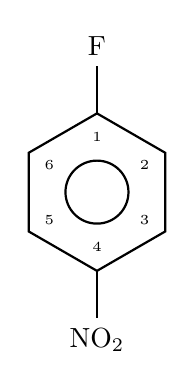
\begin{tikzpicture}[thick]
  \draw (90:1) -- (30:1) -- (-30:1) -- (-90:1) -- (-150:1) -- (150:1) -- cycle;
  \draw (0,0) circle (4mm);
  \foreach \k/\lab in {90/1,30/2,-30/3,-90/4,-150/5,150/6} \node[font=\tiny] at (\k:7mm) {\lab};
  \draw (90:1) -- ++(90:6mm) node[above] {F};
  \draw (-90:1) -- ++(-90:6mm) node[below] {NO$_2$};
\end{tikzpicture}
&
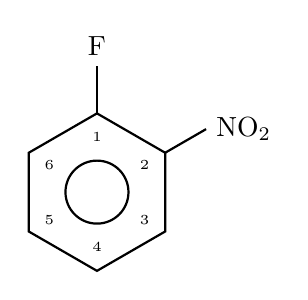
\begin{tikzpicture}[thick]
  \draw (90:1) -- (30:1) -- (-30:1) -- (-90:1) -- (-150:1) -- (150:1) -- cycle;
  \draw (0,0) circle (4mm);
  \foreach \k/\lab in {90/1,30/2,-30/3,-90/4,-150/5,150/6} \node[font=\tiny] at (\k:7mm) {\lab};
  \draw (90:1) -- ++(90:6mm) node[above] {F};
  \draw (30:1) -- ++(30:6mm) node[anchor=west] {NO$_2$};
\end{tikzpicture}
\\
para (principal, cerca de 85 a 90 %) & orto (principal, cerca de 10 a 15 %) \\
1-fluoro-4-nitrobenzeno & 1-fluoro-2-nitrobenzeno
\end{tabular}
\end{center}

\medskip
\noindent\textbf{d)} Identificação das moléculas:
\begin{itemize}
\item (i) $2\,\text{A}+1\,\text{R}=\text{H}_2\text{O}$, com $M=2\cdot1{,}01+16{,}00=18{,}02\ \text{g·mol}^{-1}$;
\item (ii) $2\,\text{A}+1\,\text{Q}=\text{H}_2\text{S}$, com $M=2\cdot1{,}01+32{,}06=34{,}08\ \text{g·mol}^{-1}$;
\item (iii) $1\,\text{X}+4\,\text{A}+1\,\text{R}=\text{CH}_3\text{OH}$ (metanol), com $M=12{,}01+4\cdot1{,}01+16{,}00=32{,}05\ \text{g·mol}^{-1}$.
\end{itemize}

\noindent A massa molar não decide a ordem. O $\text{H}_2\text{S}$ tem massa molar maior que o $\text{CH}_3\text{OH}$, mas ferve muito abaixo. A ebulição é controlada pelas forças intermoleculares, e a mais intensa aqui é a ponte de hidrogênio. Ela exige um H ligado a átomo muito eletronegativo (F, O ou N) e um átomo receptor com par isolado. Pela escala de Pauling, a diferença de eletronegatividade é $3{,}44-2{,}20=1{,}24$ na ligação O–H, enquanto na ligação S–H é $2{,}58-2{,}20=0{,}38$, o que a torna pouco polar.
\begin{itemize}
\item $\text{H}_2\text{O}$ (i): 2 ligações O–H (doadores) e 2 pares isolados no O (receptores). Forma uma rede tridimensional de pontes de hidrogênio, a mais extensa dos três casos. Ebulição a $100\,^\circ\text{C}$.
\item $\text{CH}_3\text{OH}$ (iii): 1 ligação O–H por molécula. Forma pontes de hidrogênio em cadeias, menos extensas que a rede da água, e há ainda dipolo permanente e dispersões de London. Ebulição a cerca de $65\,^\circ\text{C}$.
\item $\text{H}_2\text{S}$ (ii): a ligação S–H é pouco polar, e o S é um receptor fraco, de modo que as pontes de hidrogênio são muito fracas. Predominam dipolo permanente (molécula angular) e dispersões de London. Ebulição a cerca de $-60\,^\circ\text{C}$.
\end{itemize}

\noindent Ordem crescente de ponto de ebulição: (ii) $<$ (iii) $<$ (i), ou seja, $\text{H}_2\text{S}<\text{CH}_3\text{OH}<\text{H}_2\text{O}$. As temperaturas ($-60$, $65$ e $100\,^\circ\text{C}$) estão nessa ordem.

\medskip
\noindent ANSWER: a) 3 arranjos (átomo central C, N ou S; as 6 sequências se reduzem a 3 pela inversão); b) $\text{BF}_3$ (trigonal planar) e $\text{NH}_3$ (pirâmide trigonal); c) nitração do $\text{C}_6\text{H}_5\text{F}$ por $\text{NO}_2^{+}$: 1-fluoro-4-nitrobenzeno (para, majoritário, cerca de 85 a 90 %) e 1-fluoro-2-nitrobenzeno (orto, cerca de 10 a 15 %), com meta desprezível; d) $\text{H}_2\text{S}<\text{CH}_3\text{OH}<\text{H}_2\text{O}$, ou seja, (ii) $<$ (iii) $<$ (i).%
\newpage%
\section*{Questão 6}

\section*{Solução}

\textbf{Hipóteses.} Soluções diluídas a 25\,$^{\circ}$C e 1 atm. As atividades são aproximadas pelas concentrações em $\mathrm{mol\,L^{-1}}$ (o enunciado define o padrão como atividade unitária), e as constantes são adimensionais. As reações 1 e 2 ocorrem em meio aquoso. A reação 3 é avaliada pelo mesmo critério, com ressalva de solvente ao final. Adota-se $K_w = 1{,}0\times10^{-14}$, isto é, $pK_w = 14{,}00$. A água, como reagente e solvente, entra na constante $K_b(\mathrm{H_2O})$ da reação $\mathrm{H_2O} + \mathrm{H_2O} \rightleftharpoons \mathrm{H_3O^+} + \mathrm{OH^-}$: $K_b = [\mathrm{H_3O^+}][\mathrm{OH^-}]/[\mathrm{H_2O}] = K_w/55{,}5 \approx 1{,}8\times10^{-16}$ ($pK_b \approx 15{,}74$). Esse valor é compatível com o dado $15{,}70$, que se usa como fornecido. A mesma expressão $K_w/[\mathrm{H_2O}]$ é a constante de ionização da água, logo $pK_a(\mathrm{H_2O})$ tem o mesmo valor numérico, $15{,}70$.

\textbf{Passo 1 (pares conjugados).} Somando $\mathrm{HA} \rightleftharpoons \mathrm{H^+} + \mathrm{A^-}$ e $\mathrm{A^-} + \mathrm{H_2O} \rightleftharpoons \mathrm{HA} + \mathrm{OH^-}$, as espécies HA e A$^-$ se cancelam e resta $\mathrm{H_2O} \rightleftharpoons \mathrm{H^+} + \mathrm{OH^-}$. A constante da soma é o produto das constantes, $K_aK_b = K_w$. Em logaritmo negativo,
\[
pK_a + pK_b = pK_w = 14{,}00 .
\]

\textbf{Passo 2 (espécies não fornecidas).} Aplicando o passo 1:
\[
\begin{array}{lcc}
\text{Par conjugado} & pK_a & pK_b \\ \hline
\mathrm{CH_3C{\equiv}CH}\,/\,\mathrm{CH_3C{\equiv}C^-} & 25{,}00\ \text{(dado)} & -11{,}00 \\
\mathrm{H_3O^+}\,/\,\mathrm{H_2O} & -1{,}70 & 15{,}70\ \text{(dado)} \\
\mathrm{NH_4^+}\,/\,\mathrm{NH_3} & 9{,}25 & 4{,}75\ \text{(dado)} \\
\mathrm{NH_3}\,/\,\mathrm{NH_2^-} & 36{,}00 & -22{,}00\ \text{(dado)} \\
\mathrm{H_2O}\,/\,\mathrm{OH^-} & 15{,}70\ \text{(hipótese)} & -1{,}70
\end{array}
\]
Cálculos: $pK_b(\mathrm{CH_3C{\equiv}C^-}) = 14{,}00 - 25{,}00 = -11{,}00$; $pK_a(\mathrm{H_3O^+}) = 14{,}00 - 15{,}70 = -1{,}70$; $pK_a(\mathrm{NH_4^+}) = 14{,}00 - 4{,}75 = 9{,}25$; $pK_a(\mathrm{NH_3}) = 14{,}00 - (-22{,}00) = 36{,}00$; $pK_b(\mathrm{OH^-}) = 14{,}00 - 15{,}70 = -1{,}70$. Valores negativos são válidos: $pK < 0$ significa constante maior que 1. Por exemplo, o propinido ($pK_b = -11{,}00$) é base muito mais forte que $\mathrm{OH^-}$.

\textbf{Passo 3 (critério de equilíbrio).} Para $\mathrm{HA} + \mathrm{B} \rightleftharpoons \mathrm{A^-} + \mathrm{BH^+}$, tem-se $K = \dfrac{[\mathrm{A^-}][\mathrm{BH^+}]}{[\mathrm{HA}][\mathrm{B}]}$. Multiplicando numerador e denominador por $[\mathrm{OH^-}]$ e reagrupando,
\[
K = \frac{[\mathrm{BH^+}][\mathrm{OH^-}]}{[\mathrm{B}]}\cdot\frac{[\mathrm{A^-}]}{[\mathrm{HA}][\mathrm{OH^-}]} = \frac{K_b(\mathrm{B})}{K_b(\mathrm{A^-})}
\quad\Rightarrow\quad
\log K = pK_b(\mathrm{A^-}) - pK_b(\mathrm{B}).
\]
Assim, $K>1$ (favorece os produtos) quando $pK_b(\mathrm{A^-}) > pK_b(\mathrm{B})$, ou seja, quando a base do reagente é mais forte que a base do produto. Equivalentemente, $K = K_a(\mathrm{HA})/K_a(\mathrm{BH^+})$, o que serve de conferência.

\textbf{Passo 4 (aplicação).}

\textbf{a) Reação 1.} Aqui $\mathrm{HA} = $ propino, $\mathrm{B} = \mathrm{H_2O}$ e $\mathrm{BH^+} = \mathrm{H_3O^+}$:
\[
\log K_1 = -11{,}00 - 15{,}70 = -26{,}70
\quad\Rightarrow\quad
K_1 = 10^{-26{,}70} = 10^{0{,}30}\times10^{-27} \approx 2\times10^{-27}.
\]
Como $K_1 \ll 1$, o equilíbrio \textbf{não favorece} a formação dos produtos: a água não desprotona o propino em quantidade apreciável. Conferência: $pK_a(\mathrm{H_3O^+}) - pK_a(\mathrm{propino}) = -1{,}70 - 25{,}00 = -26{,}70$.

\textbf{b) Reação 2.} Aqui $\mathrm{B} = \mathrm{NH_3}$ e $\mathrm{BH^+} = \mathrm{NH_4^+}$:
\[
\log K_2 = -11{,}00 - 4{,}75 = -15{,}75
\quad\Rightarrow\quad
K_2 = 10^{-15{,}75} = 10^{0{,}25}\times10^{-16} \approx 1{,}8\times10^{-16}.
\]
Como $K_2 \ll 1$, o equilíbrio \textbf{não favorece} a formação dos produtos. Conferência: $pK_a(\mathrm{NH_4^+}) - pK_a(\mathrm{propino}) = 9{,}25 - 25{,}00 = -15{,}75$.

\textbf{c) Reação 3.} O $\mathrm{Na^+}$ aparece nos dois lados e é espectador. A equação iônica líquida é $\mathrm{CH_3C{\equiv}CH} + \mathrm{NH_2^-} \rightleftharpoons \mathrm{CH_3C{\equiv}C^-} + \mathrm{NH_3}$, com $\mathrm{B} = \mathrm{NH_2^-}$ e $\mathrm{BH^+} = \mathrm{NH_3}$:
\[
\log K_3 = -11{,}00 - (-22{,}00) = +11{,}00
\quad\Rightarrow\quad
K_3 = 10^{11}.
\]
Como $K_3 \gg 1$, o equilíbrio \textbf{favorece} a formação dos produtos, de modo praticamente completo. Conferência: $pK_a(\mathrm{NH_3}) - pK_a(\mathrm{propino}) = 36{,}00 - 25{,}00 = 11{,}00$.

\textbf{Ressalva de solvente (reação 3).} Os valores $pK_a = 25{,}00$ (propino) e $36{,}00$ ($\mathrm{NH_3}$) são maiores que $15{,}70$, o pK da água, ou seja, esses ácidos são mais fracos que a água. O $\mathrm{NH_2^-}$ seria destruído por ela: $\mathrm{NH_2^-} + \mathrm{H_2O} \rightleftharpoons \mathrm{NH_3} + \mathrm{OH^-}$, com $\log K = pK_b(\mathrm{OH^-}) - pK_b(\mathrm{NH_2^-}) = -1{,}70 + 22{,}00 = 20{,}30$. Portanto, a reação 3 só existe de forma apreciável em solvente não aquoso, como a amônia líquida usada no preparo de acetiletos com $\mathrm{NaNH_2}$. Nesse meio a escala de pK é outra, e $10^{11}$ vale apenas como ordem de grandeza. O sinal de $\log K$ (diferença de 11 unidades de pK) é robusto.

ANSWER: a) não favorece ($K_1 \approx 2\times10^{-27}$); b) não favorece ($K_2 \approx 1{,}8\times10^{-16}$); c) favorece ($K_3 \approx 10^{11}$).%
\newpage%
\section*{Questão 7}

\section*{Solução}

\textbf{Relações e hipóteses.} Pela relação de Planck-Einstein, um fóton de comprimento de onda $\lambda$ tem energia $E=\dfrac{hc}{\lambda}$, e um mol desses fótons tem energia $E_m=N_A\dfrac{hc}{\lambda}$. Para $\lambda=450\ \text{nm}=4{,}50\times10^{-7}\ \text{m}$:
\[
E=\frac{6{,}63\times10^{-34}\cdot 3{,}0\times10^{8}}{4{,}50\times10^{-7}}\approx 4{,}42\times10^{-19}\ \text{J}\approx 2{,}76\ \text{eV},\qquad E_m\approx 2{,}66\times10^{5}\ \text{J}\cdot\text{mol}^{-1}.
\]
Hipóteses, com origem no enunciado: (i) cada fóton absorvido gera um elétron (enunciado geral); (ii) a equação dada, com $\text{H}_2\text{O}(\ell)$, fornece $\Delta H^{\circ}=+572\ \text{kJ}$ para a reação escrita, ou seja, $+286\ \text{kJ}$ por mol de $\text{H}_2$; (iii) eficiência quântica de 100% no item (c), e ausência de perdas nos itens (d) e (e): em (d) a palavra "mínima" equivale a isso, pois qualquer perda exigiria mais fótons, e em (e) o enunciado diz "não há perdas energéticas"; (iv) a pressão de 700 bar é desprezada, como pedido em (d). Pelo balanço do item (a), 1 mol de $\text{H}_2$ consome 2 mol de elétrons e, pela hipótese (i), exige 2 mol de fótons.

\textbf{a)} A luz excita o semicondutor, que gera pares elétron-lacuna: $\text{SC}+h\nu\rightarrow e^{-}+h^{+}$. Como o semicondutor é o eletrodo fotoativo, na configuração usual (fotoânodo), as lacunas oxidam a água em sua superfície, liberando $\text{O}_2$. Os elétrons percorrem o circuito externo até o cátodo (eletrodo auxiliar), onde reduzem $\text{H}^{+}$ a $\text{H}_2$. Em meio ácido:
\[
\text{Cátodo (redução):}\quad 2\text{H}^{+}(aq)+2e^{-}\rightarrow\text{H}_2(g)
\]
\[
\text{Ânodo (oxidação):}\quad \text{H}_2\text{O}(\ell)\rightarrow\tfrac{1}{2}\text{O}_2(g)+2\text{H}^{+}(aq)+2e^{-}
\]
Conferência: multiplicando ambas por 2 e somando, cancelam-se $4\text{H}^{+}$ e $4e^{-}$, restando $2\text{H}_2\text{O}(\ell)\rightarrow 2\text{H}_2(g)+\text{O}_2(g)$, a equação dada, com balanço de massa e de carga. Em meio básico, de forma equivalente: cátodo $2\text{H}_2\text{O}(\ell)+2e^{-}\rightarrow\text{H}_2(g)+2\text{OH}^{-}(aq)$ e ânodo $2\text{OH}^{-}(aq)\rightarrow\tfrac{1}{2}\text{O}_2(g)+\text{H}_2\text{O}(\ell)+2e^{-}$.

\textbf{b)} Para 1 mol de $\text{H}_2$ são necessários 2 mol de elétrons, logo são absorvidos 2 mol de fótons de 450 nm. A energia fornecida pela luz é a soma das energias desses fótons:
\[
E_{\text{luz}}=2\cdot 2{,}66\times10^{5}\ \text{J}=5{,}32\times10^{5}\ \text{J}\ (=532\ \text{kJ}).
\]
Parte dessa energia fica armazenada como energia química: $286\ \text{kJ}$ por mol de $\text{H}_2$, ou $143\ \text{kJ}$ por mol de elétrons, que equivalem a $2{,}38\times10^{-19}\ \text{J}\approx 1{,}48$ eV por elétron. Cada fóton fornece $2{,}76$ eV, e o excesso, cerca de $1{,}28$ eV por elétron, é dissipado. Como $\Delta H^{\circ}$ é o único dado termoquímico da prova, esta comparação é apenas uma estimativa. O critério termodinâmico rigoroso seria $\Delta G^{\circ}$, que não é fornecido.

\textbf{c)} Com $P=10\ \text{W}\cdot\text{m}^{-2}$, $A=0{,}2\ \text{m}^{2}$ e $t=3600\ \text{s}$, a potência total incidente é $P\cdot A$ (pois $\text{W}=\text{J}\cdot\text{s}^{-1}$), e a energia recebida é:
\[
E_{\text{luz}}=P\cdot A\cdot t=10\cdot 0{,}2\cdot 3600\ \text{J}=7{,}2\times10^{3}\ \text{J}.
\]
Com $\eta=100\%$ e proporção 1:1, o número de elétrons é igual ao de fótons: $n_{e^-}=\dfrac{7{,}2\times10^{3}}{2{,}66\times10^{5}}\approx 2{,}71\times10^{-2}$ mol. Como cada $\text{H}_2$ consome 2 elétrons:
\[
n_{\text{H}_2}=\frac{n_{e^-}}{2}=\frac{7{,}2\times10^{3}}{2\cdot 2{,}66\times10^{5}}\approx 1{,}35\times10^{-2}\ \text{mol}\qquad(\approx 0{,}027\ \text{g de H}_2).
\]

\textbf{d)} Com $M(\text{H}_2)=2\times1{,}01=2{,}02\ \text{g}\cdot\text{mol}^{-1}$ e $5{,}65\ \text{kg}=5650\ \text{g}$:
\[
n_{\text{H}_2}=\frac{5650\ \text{g}}{2{,}02\ \text{g}\cdot\text{mol}^{-1}}\approx 2{,}797\times10^{3}\ \text{mol}.
\]
O pedido é a "energia mínima necessária para gerar essa quantidade de gás pela fotodecomposição da água, utilizando o semicondutor", isto é, a energia luminosa absorvida. É a mesma grandeza do item (b), escalada para a massa do tanque. O semicondutor absorve luz com comprimento de onda $\lambda\le 450$ nm, pois 450 nm é o máximo (limiar). Logo todo fóton absorvido tem $E=hc/\lambda\ge 4{,}42\times10^{-19}\ \text{J}$, e o de menor energia absorvível é o de 450 nm. Como cada $\text{H}_2$ exige 2 fótons absorvidos, e com $\eta=100\%$ para que a energia seja mínima:
\[
E_{\min}=n_{\text{H}_2}\cdot\left(2\cdot 2{,}66\times10^{5}\ \text{J}\right)=2{,}797\times10^{3}\cdot 5{,}32\times10^{5}\ \text{J}\approx 1{,}49\times10^{9}\ \text{J}.
\]
Por que não a energia química? A energia química armazenada, $n_{\text{H}_2}\cdot 286\ \text{kJ}\cdot\text{mol}^{-1}\approx 8{,}00\times10^{8}\ \text{J}$, seria o mínimo apenas se o semicondutor absorvesse fótons de $1{,}48$ eV por elétron. Como seu limiar corresponde a $2{,}76$ eV, a energia luminosa exigida é a dos fótons de 450 nm. A diferença, $\approx 6{,}9\times10^{8}\ \text{J}$, é o excesso dissipado, como em (b). Esse valor químico é a grandeza usada em (e), não a pedida aqui.

A pressão de 700 bar só alteraria a energia química, por meio do termo $RT\ln(p/p^{\circ})\approx 16\ \text{kJ}\cdot\text{mol}^{-1}$ da energia de Gibbs do $\text{H}_2$ a 298 K, e do trabalho de compressão. O enunciado manda desprezá-lo, e a energia dos fótons não depende da pressão: a massa serve apenas para contar mols.

\textbf{e)} A combustão é o inverso da decomposição, dividido por 2 para 1 mol de $\text{H}_2$: $\text{H}_2(g)+\tfrac{1}{2}\text{O}_2(g)\rightarrow\text{H}_2\text{O}(\ell)$, com $\Delta H^{\circ}=-286\ \text{kJ}\cdot\text{mol}^{-1}$. Logo:
\[
E_{\text{comb}}=2{,}797\times10^{3}\ \text{mol}\cdot 286\ \text{kJ}\cdot\text{mol}^{-1}\approx 8{,}00\times10^{5}\ \text{kJ}=8{,}00\times10^{8}\ \text{J}.
\]
Sem perdas, a energia luminosa total iguala $E_{\text{comb}}$. Com proporção 1:1 e 2 elétrons por $\text{H}_2$, são necessários $n_{\text{fótons}}=2\,n_{\text{H}_2}\approx 5{,}594\times10^{3}$ mol de fótons. A energia molar do fóton é:
\[
E_m=\frac{E_{\text{comb}}}{n_{\text{fótons}}}=\frac{8{,}00\times10^{8}\ \text{J}}{5{,}594\times10^{3}\ \text{mol}}\approx 1{,}43\times10^{5}\ \text{J}\cdot\text{mol}^{-1}=\frac{286\ \text{kJ}\cdot\text{mol}^{-1}}{2},
\]
que não depende da massa de $\text{H}_2$. Com $E_m=N_A\dfrac{hc}{\lambda_{\max}}$, isola-se $\lambda_{\max}=\dfrac{N_A\,h\,c}{E_m}$. O numerador é:
\[
N_A\,h\,c=6{,}02\times10^{23}\cdot 6{,}63\times10^{-34}\cdot 3{,}0\times10^{8}=39{,}91\times10^{-11}\cdot 3{,}0\times10^{8}\approx 1{,}197\times10^{-1}\ \text{J}\cdot\text{m}\cdot\text{mol}^{-1}.
\]
Logo:
\[
\lambda_{\max}=\frac{1{,}197\times10^{-1}\ \text{J}\cdot\text{m}\cdot\text{mol}^{-1}}{1{,}43\times10^{5}\ \text{J}\cdot\text{mol}^{-1}}\approx 8{,}37\times10^{-7}\ \text{m}=837\ \text{nm}.
\]
Unidades: $(\text{J}\cdot\text{m}\cdot\text{mol}^{-1})/(\text{J}\cdot\text{mol}^{-1})=\text{m}$. Como $E\propto 1/\lambda$, fótons com $\lambda\le 837$ nm (infravermelho próximo) têm energia suficiente, e 837 nm é o limite superior.

Conferências:
(i) Por escala, independente da fórmula de $N_A$: $\lambda_{\max}=450\ \text{nm}\cdot\dfrac{E(450\ \text{nm})}{E_{\text{necessária}}}=450\cdot\dfrac{4{,}42}{2{,}38}\approx 450\cdot 1{,}86\approx 837$ nm, com $E_{\text{necessária}}=2{,}38\times10^{-19}\ \text{J}\approx 1{,}48$ eV por fóton.
(ii) Consistência com (d): $\dfrac{1{,}49\times10^{9}}{8{,}00\times10^{8}}\approx 1{,}86$, igual à razão $\dfrac{4{,}42}{2{,}38}\approx 1{,}86$ entre as energias por elétron, como deve ser.
(iii) Fator 2: se o fator 2 de elétrons fosse esquecido (1 fóton por $\text{H}_2$), $\lambda$ seria $\approx 419$ nm. Essa resposta é rejeitada, pois 1 mol de $\text{H}_2$ exige 2 mol de elétrons, e a proporção 1:1 vale entre elétrons e fótons.

ANSWER: a) cátodo: $2\text{H}^{+}+2e^{-}\rightarrow\text{H}_2$; ânodo: $\text{H}_2\text{O}\rightarrow\tfrac{1}{2}\text{O}_2+2\text{H}^{+}+2e^{-}$; b) $5{,}32\times10^{5}$ J (532 kJ); c) $1{,}35\times10^{-2}$ mol de $\text{H}_2$; d) $1{,}49\times10^{9}$ J; e) $\lambda_{\max}\approx 837$ nm
%
\newpage%
\section*{Questão 8}

\section*{Solução}

\textbf{Hipóteses gerais.} (i) Combustão completa e estequiométrica: todo o CH$_4$ queimado é consumido. (ii) Entalpias de formação e calor específico independentes de $T$ e $P$, como informa o enunciado. (iii) Pelo requisito I, os produtos são gasosos, inclusive a água. (iv) Massas molares: $M(\mathrm{CH_4})=16{,}05$, $M(\mathrm{O_2})=32{,}00$, $M(\mathrm{CO_2})=44{,}01$ e $M(\mathrm{H_2O})=18{,}02\ \text{g}\cdot\text{mol}^{-1}$.

\textbf{a)} Balanceamento pela conservação dos átomos: C: $1=1$; H: $4=2\cdot2$; O: $2\cdot2=2+2$. Logo:

\[ \mathrm{CH_4(g)}+2\,\mathrm{O_2(g)}\rightarrow\mathrm{CO_2(g)}+2\,\mathrm{H_2O(g)} \]

Como o requisito I exige apenas produtos gasosos, a água formada é vapor. A tabela fornece $\mathrm{H_2O(\ell)}$, então corrige-se pela vaporização, $\mathrm{H_2O(\ell)}\rightarrow\mathrm{H_2O(g)}$ com $\Delta H=+45\ \text{kJ}\cdot\text{mol}^{-1}$. Pela lei de Hess:

\[ \Delta H_f[\mathrm{H_2O(g)}]=-286+45=-241\ \text{kJ}\cdot\text{mol}^{-1} \]

Pela lei de Hess, $\Delta H_c=\sum n\,\Delta H_f(\text{produtos})-\sum n\,\Delta H_f(\text{reagentes})$, com $\Delta H_f[\mathrm{O_2(g)}]=0$ por ser substância simples no estado padrão:

\begin{align*}
\Delta H_c &= \big[-393+2(-241)\big]-\big[-75+2\cdot0\big]\\
&= -875+75=-800\ \text{kJ}\cdot\text{mol}^{-1}
\end{align*}

O sinal negativo indica reação exotérmica: cada mol de CH$_4$ queimado libera $800\ \text{kJ}$. Conferência: o valor tabelado para a água gasosa é da ordem de $-802\ \text{kJ}\cdot\text{mol}^{-1}$. Usar $\mathrm{H_2O(\ell)}$ daria $-890\ \text{kJ}\cdot\text{mol}^{-1}$, o que contraria o requisito I.

\textbf{b)} O requisito I fixa $Q=12\ \text{MJ}=12\,000\ \text{kJ}$. Pela estequiometria $1:2$:

\[ n_{\mathrm{CH_4}}=\frac{12\,000\ \text{kJ}}{800\ \text{kJ}\cdot\text{mol}^{-1}}=15\ \text{mol}\qquad n_{\mathrm{O_2}}=2\cdot15=30\ \text{mol} \]

\[ m_{\mathrm{CH_4}}=15\cdot16{,}05=240{,}75\ \text{g}\qquad m_{\mathrm{O_2}}=30\cdot32{,}00=960\ \text{g} \]

Conservação de massa: reagentes $240{,}75+960=1\,200{,}75\ \text{g}$; produtos $15\cdot44{,}01+30\cdot18{,}02=660{,}15+540{,}60=1\,200{,}75\ \text{g}$. Ordem de grandeza: $12\,000\ \text{kJ}/240{,}75\ \text{g}\approx49{,}8\ \text{kJ}\cdot\text{g}^{-1}$, compatível com o metano (cerca de 50 kJ/g).

\textbf{c)} Interpretação dos dados. A "câmara de combustão" do requisito I é a câmara principal: é nela que o metano gasoso é injetado (requisito II), e é dela que a tubeira absorve calor. A pré-câmara é tratada à parte no requisito III. Assim:
\begin{itemize}
\item os $12$ MJ e os $15$ mol do item b correspondem à câmara principal;
\item a turbobomba "pressuriza o combustível a ser queimado na câmara principal", ou seja, $240{,}75\ \text{g}$;
\item o metano da pré-câmara, de massa $m_p$ (quantidade $n_p$), é suprido à parte. Não entra na massa pressurizada pela bomba, pois o enunciado atribui a ela só o combustível da câmara principal. Seu calor de combustão é o do requisito III, que não entra nos $12$ MJ.
\end{itemize}

Na pré-câmara o CH$_4$ queima por completo, e a entalpia por mol não depende do excesso de O$_2$, logo $Q_p=800\ \text{kJ}\cdot\text{mol}^{-1}\cdot n_p$. A energia útil da bomba deve igualar a energia exigida:

\begin{align*}
Q_p &= 800\ \text{kJ}\cdot\text{mol}^{-1}\cdot n_p = 8{,}00\times10^{5}\,n_p\ \text{J}\\
0{,}30\,Q_p &= 2{,}40\times10^{5}\,n_p\ \text{J}\\
E_{\text{exigida}} &= 40\ \text{J}\cdot\text{g}^{-1}\cdot240{,}75\ \text{g}=9\,630\ \text{J}
\end{align*}

\begin{align*}
2{,}40\times10^{5}\,n_p &= 9\,630\\
n_p &= \frac{9\,630}{240\,000}=0{,}040125\ \text{mol}
\end{align*}

\[ m_p=n_p\,M(\mathrm{CH_4})=0{,}040125\cdot16{,}05\approx0{,}644\ \text{g} \]

Verificação: $Q_p=800\cdot0{,}040125=32{,}1\ \text{kJ}$; $30\%$ disso são $9{,}63\ \text{kJ}=9\,630\ \text{J}=40\ \text{J}\cdot\text{g}^{-1}\times240{,}75\ \text{g}$. A fração $0{,}644/240{,}75\approx0{,}27\%$ é uma "pequena porcentagem", como descrito no enunciado.

Sensibilidade à interpretação: se os $15$ mol totais incluíssem o metano da pré-câmara, a bomba pressurizaria $(15-n_p)$ mol e a equação seria $240\,000\,n_p=642\,(15-n_p)$, com $642=40\cdot16{,}05$. Obtém-se $n_p=0{,}040018$ mol e $m_p=0{,}642\ \text{g}$. Ambos os valores arredondam para $0{,}64\ \text{g}$ com dois algarismos significativos.

\textbf{d)} Calor absorvido pela tubeira (requisito II):
\[ Q_T=0{,}25\%\cdot12\ \text{MJ}=0{,}0025\cdot1{,}2\times10^{7}\ \text{J}=3{,}0\times10^{4}\ \text{J} \]

Hipóteses: todo $Q_T$ é transferido ao CH$_4(\ell)$, sem perdas. O metano permanece líquido durante o aquecimento de $98\ \text{K}$ a $188\ \text{K}$, com $c=\tfrac{5}{3}\ \text{J}\cdot\text{g}^{-1}\cdot\text{K}^{-1}$ constante, convenção do enunciado. A mudança de fase não custa energia, como ele informa. A variação de temperatura é $\Delta T=188-98=90\ \text{K}$ (a diferença em kelvin é igual à diferença em graus Celsius).

Como $Q=m\,c\,\Delta T$, para que a temperatura não ultrapasse $188\ \text{K}$ é preciso $\Delta T\le90\ \text{K}$, logo $m\ge Q_T/(c\,\Delta T)$. A massa mínima corresponde a $\Delta T=90\ \text{K}$:

\[ m_{\min}=\frac{Q_T}{c\,\Delta T}=\frac{3{,}0\times10^{4}\ \text{J}}{\tfrac{5}{3}\ \text{J}\cdot\text{g}^{-1}\cdot\text{K}^{-1}\cdot90\ \text{K}}=\frac{3{,}0\times10^{4}}{150}\ \text{g}=200\ \text{g} \]

Verificação: $200\cdot\tfrac{5}{3}\cdot90=3{,}0\times10^{4}\ \text{J}$. Fechamento com o item c: a bomba entrega $240{,}75\ \text{g}$ pressurizados. Desses, $200\ \text{g}$ passam pelo circuito de resfriamento e são injetados como gás na câmara principal, e os $40{,}75\ \text{g}$ restantes vão diretamente à injeção. Como $200<240{,}75$, o resfriamento é viável.

ANSWER: a) $\mathrm{CH_4(g)}+2\,\mathrm{O_2(g)}\rightarrow\mathrm{CO_2(g)}+2\,\mathrm{H_2O(g)}$, $\Delta H_c=-800\ \text{kJ}\cdot\text{mol}^{-1}$; b) $240{,}75\ \text{g}$ de CH$_4$ (cerca de $241\ \text{g}$) e $960\ \text{g}$ de O$_2$; c) $\approx0{,}644\ \text{g}$ de CH$_4(g)$ na pré-câmara (cerca de $0{,}64\ \text{g}$); d) $200\ \text{g}$ de CH$_4(\ell)$.%
\newpage%
\section*{Questão 9}

\section*{Solução}

\textbf{Hipóteses e dados.}
\begin{itemize}
\item Os eletrodos de platina são inertes: apenas transferem elétrons.
\item Pela Figura (A), os eletrodos ficam na zona incolor de $\mathrm{H_2SO_4}$, acima da mistura. A eletrólise dura um tempo finito, então a separação dos íons é parcial.
\item As concentrações não são dadas no enunciado, e a conclusão não depende delas. Os potenciais usam $E^\circ$, a equação de Nernst a $25\,^\circ\mathrm{C}$ (termo $0{,}059/n$ V) e $p_{\mathrm{H_2}}=p_{\mathrm{O_2}}=1$ bar.
\item Valores de tabela, externos à prova e usados apenas como ordem de grandeza: $K_{a2}(\mathrm{HSO_4^-})\approx 1{,}2\times10^{-2}$; $K=[\mathrm{HCrO_4^-}]^2/[\mathrm{Cr_2O_7^{2-}}]\approx 2\times10^{-2}$; $\mathrm{p}K_a(\mathrm{HCrO_4^-})\approx 6{,}5$; condutividades iônicas limite $\lambda^\circ(\mathrm{H^+})\approx 350$, $\lambda^\circ(\mathrm{K^+})\approx 74$ e $\lambda^\circ(\tfrac12\mathrm{Cu^{2+}})\approx 54\ \mathrm{S\,cm^2\,mol^{-1}}$.
\end{itemize}

\textbf{a) Espécies iônicas.} Dissociações e equilíbrios:
\[
\mathrm{CuSO_4 \rightarrow Cu^{2+} + SO_4^{2-}},\qquad
\mathrm{K_2Cr_2O_7 \rightarrow 2\,K^+ + Cr_2O_7^{2-}},\qquad
\mathrm{H_2SO_4 \rightarrow H^+ + HSO_4^-}
\]
\[
\mathrm{HSO_4^- \rightleftharpoons H^+ + SO_4^{2-}},\qquad
\mathrm{Cr_2O_7^{2-} + H_2O \rightleftharpoons 2\,HCrO_4^-},\qquad
\mathrm{HCrO_4^- \rightleftharpoons H^+ + CrO_4^{2-}}
\]
\begin{itemize}
\item Espécies principais: $\mathrm{Cu^{2+}}$, $\mathrm{K^+}$, $\mathrm{H^+}$, $\mathrm{SO_4^{2-}}$, $\mathrm{HSO_4^-}$, $\mathrm{Cr_2O_7^{2-}}$ e $\mathrm{HCrO_4^-}$. Para uma concentração ilustrativa de dicromato de $10^{-2}\ \mathrm{mol\,L^{-1}}$, o equilíbrio dá $[\mathrm{HCrO_4^-}]\approx 1\times10^{-2}\ \mathrm{mol\,L^{-1}}$, ou seja, cerca de metade do Cr(VI) está nessa forma.
\item Traços: $\mathrm{CrO_4^{2-}}$, com $[\mathrm{CrO_4^{2-}}]/[\mathrm{HCrO_4^-}]=10^{\mathrm{pH}-6{,}5}\le 10^{-3{,}5}$ para pH $\le 3$; e $\mathrm{OH^-}$, com $[\mathrm{OH^-}]=10^{-14}/[\mathrm{H^+}]\le 10^{-8}\ \mathrm{mol\,L^{-1}}$ para pH $\le 6$.
\end{itemize}
A acidez mantém o Cr(VI) como $\mathrm{Cr_2O_7^{2-}}$ (laranja). Em pH básico, o $\mathrm{CrO_4^{2-}}$ (amarelo) predominaria.

\textbf{b) Origem das camadas.} Sob o campo, cátions migram para o cátodo e ânions para o ânodo. O $\mathrm{Cu^{2+}}$ (azul) sobe o braço esquerdo, e o $\mathrm{Cr_2O_7^{2-}}$ (laranja) sobe o braço direito; logo, $\mathrm{Pt_1}$ é o cátodo e $\mathrm{Pt_2}$ é o ânodo (item c). Os eletrodos estão na zona de $\mathrm{H_2SO_4}$, onde só $\mathrm{H^+}$ e $\mathrm{H_2O}$ reagem: os íons coloridos não são descarregados nem reagem, apenas migram. Como a migração é parcial após um tempo finito, cada braço fica com uma faixa colorida separada da zona incolor por uma fronteira. No braço do cátodo, $\mathrm{H^+}$ e $\mathrm{K^+}$, mais móveis que o $\mathrm{Cu^{2+}}$, avançam e deixam o azul para trás, com fronteira nítida. No braço do ânodo, o $\mathrm{Cr_2O_7^{2-}}$ forma a faixa laranja; a posição exata da fronteira depende de mobilidades que o enunciado não fornece, e a explicação não depende dela. O fundo permanece marrom porque ainda contém os dois íons: a eletrólise não esvaziou a mistura original, e a cor marrom é a soma do azul com o laranja.

\textbf{c) Ânodo, cátodo e semirreações.} $\mathrm{Pt_1}$ está no braço para onde migram os cátions, e $\mathrm{Pt_2}$ está no braço dos ânions. Portanto, \textbf{$\mathrm{Pt_1}$ é o cátodo} e \textbf{$\mathrm{Pt_2}$ é o ânodo}.

\textit{Cátodo ($\mathrm{Pt_1}$, redução).} Espécies na zona do eletrodo: $\mathrm{H^+}$, $\mathrm{H_2O}$, $\mathrm{K^+}$ e $\mathrm{SO_4^{2-}}$. O $\mathrm{K^+}$ ($E^\circ\approx -2{,}93$ V) não se reduz em água, e o enxofre do sulfato já está em +6. O $\mathrm{H^+}$ é a espécie redutível de maior potencial:
\[
\mathrm{2\,H^+(aq) + 2\,e^- \rightarrow H_2(g)}\qquad E=-\frac{0{,}059}{2}\log\frac{1}{[\mathrm{H^+}]^2}=-0{,}059\,\mathrm{pH}\ \mathrm{V}
\]
A forma $\mathrm{2\,H_2O + 2\,e^- \rightarrow H_2 + 2\,OH^-}$ tem o mesmo potencial de equilíbrio; em meio ácido, usa-se a forma com $\mathrm{H^+}$.

\textit{Condição de validade.} Se $\mathrm{Cu^{2+}}$ ($E^\circ=+0{,}34$ V) ou $\mathrm{Cr_2O_7^{2-}}$ ($E^\circ=+1{,}33$ V) chegassem ao cátodo, seriam reduzidos antes do $\mathrm{H^+}$. Na Figura (B), eles não chegam, pois ficam fora da zona do eletrodo.

\textit{Ânodo ($\mathrm{Pt_2}$, oxidação).} Espécies na zona do eletrodo: $\mathrm{H_2O}$, $\mathrm{H^+}$ e $\mathrm{SO_4^{2-}}$. Cu(II) e Cr(VI) não se oxidam em condições normais. O sulfato poderia gerar persulfato ($\mathrm{S_2O_8^{2-}}$, $E^\circ=2{,}01$ V), mas esse processo exige $\mathrm{H_2SO_4}$ concentrado e alta densidade de corrente, condições ausentes aqui. A água tem potencial bem menor e é oxidada:
\[
\mathrm{2\,H_2O(\ell) \rightarrow O_2(g) + 4\,H^+(aq) + 4\,e^-}
\]
O potencial de equilíbrio da semirreação escrita como redução é $E(\mathrm{O_2/H_2O})=1{,}23-0{,}059\,\mathrm{pH}$ V.

\textit{Balanceamento.} Multiplica-se a semirreação catódica por 2 para igualar os 4 elétrons:
\[
\mathrm{4\,H^+ + 4\,e^- \rightarrow 2\,H_2}\quad(\times 2)\qquad\Rightarrow\qquad \mathrm{2\,H_2O \rightarrow 2\,H_2 + O_2}
\]

\textit{Checagem termodinâmica.} $E^\circ_{\mathrm{cél}}=E^\circ_{\mathrm{cát}}-E^\circ_{\mathrm{an}}=0-1{,}23=-1{,}23$ V. Como os dois potenciais variam igualmente com o pH, a diferença é $1{,}23$ V em qualquer pH. Então:
\[
\Delta G^\circ=-nF\,E^\circ_{\mathrm{cél}}=-4\times 9{,}65\times10^{4}\times(-1{,}23)\ \mathrm{J\,mol^{-1}}\approx +4{,}75\times10^{5}\ \mathrm{J\,mol^{-1}}>0
\]
O processo não é espontâneo. A fonte deve fornecer mais que $1{,}23$ V, além das sobretensões (sobretudo a do $\mathrm{O_2}$) e da queda ôhmica. São 4 H$^+$ produzidos no ânodo e 4 consumidos no cátodo: a acidez global não muda, e o H$^+$ apenas migra do ânodo para o cátodo. Com 2 elétrons por H$_2$ e 4 por O$_2$, o volume de H$_2$ é o dobro do de O$_2$ nas mesmas condições.

\textbf{d) Polaridade e corrente.} Pela Figura (A), o fio de $\mathrm{P_1}$ liga-se a $\mathrm{Pt_1}$ (cátodo), e o de $\mathrm{P_2}$ liga-se a $\mathrm{Pt_2}$ (ânodo), sem cruzamento.
\begin{itemize}
\item $\mathrm{P_1}$ é o polo \textbf{negativo}, pois fornece elétrons ao cátodo. $\mathrm{P_2}$ é o polo \textbf{positivo}, pois recebe elétrons do ânodo.
\item Sentido convencional da corrente: $\mathrm{P_2 \rightarrow Pt_2}$ pelo fio; na solução, de $\mathrm{Pt_2}$ para $\mathrm{Pt_1}$, isto é, da direita para a esquerda; $\mathrm{Pt_1 \rightarrow P_1}$ pelo fio; e, dentro da fonte, de $\mathrm{P_1}$ para $\mathrm{P_2}$.
\item Na solução, os cátions se deslocam para a esquerda e os ânions para a direita. Ambos transportam corrente no mesmo sentido, da direita para a esquerda. Nos fios, os elétrons vão em sentido oposto: de $\mathrm{P_1}$ para $\mathrm{Pt_1}$ e de $\mathrm{Pt_2}$ para $\mathrm{P_2}$.
\end{itemize}

ANSWER: a) $\mathrm{Cu^{2+}}$, $\mathrm{K^+}$, $\mathrm{H^+}$, $\mathrm{SO_4^{2-}}$, $\mathrm{HSO_4^-}$, $\mathrm{Cr_2O_7^{2-}}$ e $\mathrm{HCrO_4^-}$, com $\mathrm{CrO_4^{2-}}$ e $\mathrm{OH^-}$ em traços; b) os íons coloridos migram para os eletrodos de sinal oposto, sem descarga na zona de $\mathrm{H_2SO_4}$, e as faixas se formam pela migração parcial; c) $\mathrm{Pt_1}$ é o cátodo, com $\mathrm{2H^+ + 2e^- \rightarrow H_2}$, e $\mathrm{Pt_2}$ é o ânodo, com $\mathrm{2H_2O \rightarrow O_2 + 4H^+ + 4e^-}$; d) $\mathrm{P_1}$ é negativo e $\mathrm{P_2}$ é positivo, e a corrente convencional vai de $\mathrm{P_2}$ por $\mathrm{Pt_2}$, pela solução da direita para a esquerda, até $\mathrm{Pt_1}$ e $\mathrm{P_1}$.%
\newpage%
\section*{Questão 10}

\section*{Solução}

\textbf{Notação e premissas.} No símbolo ${}^{X}_{Z}\mathrm{A}$ do enunciado, $X$ é o número de massa e $Z$ é o número de prótons do elemento A; esses são os valores pedidos nos itens a) e b). Para os demais elementos, $M_Y$, $Z_Y$ e $N_Y = M_Y - Z_Y$ são, respectivamente, o número de massa, o número de prótons e o número de nêutrons. Premissa de leitura: os valores 238 e 232 são tomados como números de massa inteiros, que é a grandeza usada nos balanços de decaimento. Em cada decaimento valem a conservação do número de massa (soma de $M$ dos reagentes igual à dos produtos) e a conservação da carga nuclear, isto é, do número atômico (soma de $Z$).

Partículas envolvidas:
\begin{itemize}
\item Alfa, ${}^{4}_{2}\mathrm{He}$: $\Delta M = -4$ e $\Delta Z = -2$.
\item Beta negativo, ${}^{0}_{-1}\mathrm{e}^{-}$: um nêutron se converte em próton, com emissão de elétron e antineutrino do elétron; $\Delta M = 0$ e $\Delta Z = +1$.
\end{itemize}
Isóbaros têm o mesmo $M$ e $Z$ diferente. Isótonos têm o mesmo $N$.

\textbf{Passo 1: identificar Q e G.} Q tem $M = 232$ e $Z = 89$, ou seja, é o actínio-232, ${}^{232}_{89}\mathrm{Ac}$. Pela consideração iii), G é produzido pela emissão beta de Q:
\[
{}^{232}_{89}\mathrm{Ac} \longrightarrow {}^{M_G}_{Z_G}\mathrm{G} + {}^{0}_{-1}\mathrm{e}^{-} + {}^{0}_{0}\overline{\nu}_{e}
\]
Conservação de $M$: $232 = M_G + 0$, logo $M_G = 232$. Conservação de $Z$: $89 = Z_G + (-1)$, logo $Z_G = 90$, que é o tório, Th. Portanto
\[
N_G = M_G - Z_G = 232 - 90 = 142.
\]

\textbf{Passo 2: identificar E.} Pela consideração iv), $Z_E = 84$, que é o polônio, Po. Pela consideração ii), E é isótono de G, então a igualdade vale para nêutrons, não para prótons: $N_E = N_G = 142$ (e não $Z_G = 90$). Logo
\[
M_E = Z_E + N_E = 84 + 142 = 226,
\]
e E é ${}^{226}_{84}\mathrm{Po}$.

\textbf{Passo 3: determinar X.} Pela consideração i), A é isóbaro de E: tem o mesmo número de massa e número de prótons diferente. Logo
\[
X = M_E = 226.
\]

\textbf{Passo 4: determinar n.} J tem $M_J = 238$ e $Z_J = 92$, ou seja, é o urânio, ${}^{238}_{92}\mathrm{U}$. Seja $n$ o número de partículas alfa emitidas por J. A equação é
\[
{}^{238}_{92}\mathrm{U} \longrightarrow n\,{}^{4}_{2}\mathrm{He} + {}^{X}_{Z}\mathrm{A}.
\]
Conservação de $M$: $238 = 4n + X = 4n + 226$, logo $4n = 12$ e $n = 3$. A emissão beta não altera $M$, portanto este resultado não depende de haver betas na cadeia.

\textbf{Passo 5: determinar Z.} Aqui entra uma leitura do enunciado. Tomamos "J sofre decaimentos de partículas alfa e forma A" como descrição completa da cadeia de J, isto é, sem emissões beta. Conservação de $Z$:
\[
92 = 2n + Z \quad\Rightarrow\quad Z = 92 - 2 \cdot 3 = 86.
\]
Se J tivesse $k$ emissões beta, a mesma conta daria $Z = 86 + k$. O enunciado não menciona emissões beta para J, por isso adotamos $k = 0$. O elemento de número atômico 86 é o radônio, Rn, logo A é ${}^{226}_{86}\mathrm{Rn}$.

\textbf{Passo 6: verificação.} A equação balanceada é
\[
{}^{238}_{92}\mathrm{U} \longrightarrow 3\,{}^{4}_{2}\mathrm{He} + {}^{226}_{86}\mathrm{Rn}.
\]
Conservação de $M$: $3 \cdot 4 + 226 = 238$. Conservação de $Z$: $3 \cdot 2 + 86 = 92$. Além disso, $Z_A = 86 \neq 84 = Z_E$, de modo que A e E são elementos distintos com o mesmo número de massa, como define a consideração i).

Checagem de consistência (não é prova): se a emissão beta de Q fosse ignorada e usássemos $Z_G = 89$, teríamos $N_G = 143$, $M_E = 227$ e $4n = 238 - 227 = 11$, sem solução inteira. Logo o resultado depende da etapa beta.

Sinais e unidades: os sinais de $\Delta Z$ (-2 para a alfa, +1 para o beta negativo) foram usados nos balanços acima. $M$, $Z$, $N$ e $n$ são contagens inteiras, sem unidade. Ordens de grandeza não se aplicam, pois não há grandeza física contínua envolvida.

\textbf{Resultado.} Admitindo que as únicas emissões de J são alfa, o urânio-238 emite $n = 3$ partículas alfa e forma o radônio-226 (A), com $X = 226$ e $Z = 86$.

ANSWER: a) X = 226; b) Z = 86 (A = Rn-226, supondo que as únicas emissões de J são alfa); c) 3 partículas alfa.%
\newpage%
\section*{Apêndice: parecer do avaliador}%
\subsection*{Questão 1: nota 9,0 (aprovada, rodada 1 de 1)}%
\textbf{Resposta da resolução às cegas do avaliador:} a) {[}HA{]} na Solução 2 = 0,40 mol/L\newline%
b) {[}HA{]} na Solução 1 = 2,0 mol/L\newline%
c) {[}base{]} na Solução 3 = 2/95 $\approx$ 2,1 $\times$ 10\^{}{-}2 mol/L ($\approx$ 0,021 mol/L)\newline%
\newline%
Resumo do raciocínio: a diluição 4 mL $\to$ 20 mL é de fator 5 (C1 = 5$\cdot$C2). No equivalente, n(HA) = n(OH{-}) = 0,80 mmol, em 40 mL de mistura, o que dá {[}A{-}{]} = 0,020 mol/L. Com Kb = Kw/Ka = 10\^{}{-}2 e pH 12 ({[}OH{-}{]} = 10\^{}{-}2), a hidrólise exige a equação completa (x/C0 = 0,5), que confirma C0 = 0,020 mol/L.\par %
Respostas finais: a) 0,40 mol/L; b) 2,0 mol/L; c) 2/95 $\approx$ 2,1$\times$10$^{-}$$^2$ mol/L. Coincidem item por item com a referência, e confiro que estão corretas. Conferi no enunciado original (página 3) e com python3 (scripts na pasta de trabalho). O balanço completo de hidrólise dá x = {[}OH$^{-}${]} = 10$^{-}$$^2$ com resíduo zero para C = 2$\times$10$^{-}$$^2$, c$_{2}$ = 0,40, c$_{1}$ = 2,0 e c$_{3}$ = 2/95. A condição protônica {[}OH$^{-}${]} = {[}HA{]} + {[}H?{]} com pH = pKa dá {[}HA{]} = {[}A$^{-}${]} = 10$^{-}$$^2$ e C = 2$\times$10$^{-}$$^2$ (desvio 10$^{-}$$^{1}$$^{0}$), que é o mesmo resultado por outro caminho, sem aproximação. A aproximação clássica x = $\surd$(K\_h$\cdot$C) daria pH $\approx$ 12,15 com C = 10$^{-}$$^2$, e a observação do candidato está correta. Traps: Solução I tratada como Solução 1; diluição de fator 5 correta; 38 mL na estequiometria e 40 mL na concentração do sal usados corretamente; K\_h = K\_w/K\_A usado; pH $\to$ {[}OH$^{-}${]} correto; aproximação rejeitada com justificativa; estequiometria 1:1; unidades e volumes corretos. Nota 9: é um gabarito publicável. Os únicos pontos a melhorar são a falta de uma frase explícita sobre a não neutralidade do equivalente e o formato LaTeX."%
\begin{itemize}%
\item%
{[}minor{]} A resolução não declara, antes das contas, que o pH do ponto de equivalência é básico porque o ânion A$^{-}$ hidrolisa (sal de ácido fraco com base forte). Isso só aparece implicitamente na condição protônica do Passo 4 e na conferência. Um gabarito comentado deveria dizer no Passo 3 por que pH 12 é consistente, e não arbitrário. Correção: acrescentar uma frase sobre a hidrólise do A$^{-}$ no Passo 3.%
\item%
{[}minor{]} A 'ordem de grandeza' da Solução 2 usa {[}H?{]} $\approx$ (K\_A$\cdot$c$_{2}$)\^{}$\frac12$ e ignora a água. Verifiquei que o efeito é desprezível: Kw/{[}H?{]} $\approx$ 1,6$\times$10$^{-}$$^{8}$ frente a {[}H?{]} $\approx$ 6,3$\times$10$^{-}$$^{7}$ (cerca de 2,5\%). Não é erro, mas a checagem poderia dizer explicitamente que é estimativa, ou usar {[}H?{]}$^2$ $\approx$ K\_A$\cdot$c$_{2}$ + K\_w.%
\item%
{[}minor{]} A saída está em marcação LaTeX (\textbackslash{}section*, \textbackslash{}textbf, itemize) com linha 'ANSWER:'. Para um caderno de soluções manuscrito, uma versão em texto limpo seria mais fiel ao formato da prova. Isso não afeta o conteúdo nem a nota.%
\end{itemize}%
\subsection*{Questão 2: nota 8,5 (não aprovada, rodada 3 de 3)}%
\textbf{Resposta da resolução às cegas do avaliador:} a) V(O2) $\approx$ 0,61 L ($\approx$ 612 mL), a 25 $^\circ$C e 1 atm, ao término da reação (consumo total de 0,050 mol de H2O2 $\to$ 0,025 mol de O2; V = nRT/P).\newline%
\newline%
b) {[}H2O2{]} restante em 5 min $\approx$ 0,35 mol$\cdot$L$^{-}$$^{1}$ ($\approx$ 0,354 mol$\cdot$L$^{-}$$^{1}$), pela cinética de 1ª ordem: {[}H2O2{]} = 0,5 $\times$ e\^{}(-0,0693$\times$5) = 0,5 $\times$ e\^{}(-0,3465) = 0,5 $\times$ 0,707.\newline%
\newline%
Não se trata de questão de múltipla escolha.\par %
Ambas as respostas finais coincidem com a referência e são corretas: (a) V(O2) $\approx$ 0,612 L ($\approx$ 612 mL), com n(O2) = 0,025 mol, T = 298 K e P = 1 atm; (b) {[}H2O2{]} $\approx$ 0,354 mol$\cdot$L$^{-}$$^{1}$ em 5 min, com {[}A{]}0$\cdot$e\^{}(-kt) = 0,5$\cdot$e\^{}(-0,3465). Conferi a prova (página 4), o enunciado confere e as contas da candidata estão corretas: t$\frac12$ = 10 min, 2\^{}-10 $\approx$ 0,1 \%, 0,050 mol de H2O2 $\to$ 0,9 mL de água ($\approx$ 1 \%), e a alternativa com convenção estequiométrica dá 0,25 mol$\cdot$L$^{-}$$^{1}$. As armadilhas foram tratadas: ordem deduzida pela unidade de k com a suposição de lei de potência declarada; exponencial natural; razão estequiométrica 2:1; condições 25 $^\circ$C e 1 atm (não CNTP); 'ao término' como limite; convenção de velocidade discutida; meia{-}vida; minutos sem conversão; hipóteses declaradas (volume constante, gás ideal, sem pressão de vapor nem solubilidade); catalisador afetando só k. Os problemas são pequenos: justificativa da convenção com redação exagerada, argumento de 'término' impreciso (100 min dá 611 mL e não 612 mL), e valores intermediários omitidos, contrariando a instrução 8. A resolução está perto de um gabarito publicável; com esses ajustes chegaria a 9 ou mais."\}{]}%
\begin{itemize}%
\item%
{[}minor{]} Convenção de velocidade: a frase 'A própria prova indica essa convenção' é exagerada. O enunciado não define a convenção; quem sugere v = -d{[}H2O2{]}/dt é o dado tabelado e\^{}(-0,3465) = 0,707. A resolução deveria dizer isso com precisão: pela convenção estequiométrica (v = -$\frac12$ d{[}H2O2{]}/dt), a constante efetiva seria 2k e {[}H2O2{]}(5 min) = 0,25 mol$\cdot$L$^{-}$$^{1}$ (confirmado: 0,25004). A escolha é ditada pelo dado da prova, não por convenção universal. Ajuste: reformular a frase e citar explicitamente a convenção estequiométrica como alternativa rejeitada pelo dado.%
\item%
{[}minor{]} Item (a), definição de 'término': a justificativa 'erro inferior à precisão dos dados' não se sustenta com três algarismos significativos. Em t = 100 min, n(O2) = 0,025$\cdot$(1 - 2\^{}-10) = 0,024976 mol e V = 0,61105 L $\approx$ 611 mL, enquanto o limite t$\to$$\infty$ dá 0,61164 L $\approx$ 612 mL. A resposta final (612 mL, rendimento estequiométrico total) está certa, mas o argumento deveria ser o limite exato t$\to$$\infty$ (consumo total do H2O2, n(O2) = 0,050/2 mol), sem o corte arbitrário de 100 min ou com esse corte apresentado como aproximação e com o erro corretamente declarado.%
\item%
{[}minor{]} Instrução 8 da prova (expressões numéricas resolvidas integralmente): valores intermediários não aparecem. Em (a), a linha 'V = 0,025$\cdot$8,21$\times$10$^{-}$$^2$$\cdot$298/1 L $\approx$ 0,612 L' pula o produto 0,6116 L. Em (b), '0,5$\cdot$0,707 $\approx$ 0,354' omite 0,3535 e o arredondamento para 0,354 não é registrado. O enunciado avisa que há desconto. Ajuste: escrever 0,025 $\times$ 0,0821 $\times$ 298 = 0,6116 L $\approx$ 0,612 L e 0,5 $\times$ 0,707 = 0,3535 $\approx$ 0,354 mol$\cdot$L$^{-}$$^{1}$.%
\end{itemize}%
\subsection*{Questão 3: nota 9,0 (aprovada, rodada 3 de 3)}%
\textbf{Resposta da resolução às cegas do avaliador:} a) Tempo para o início da precipitação: t $\approx$ 552 s ($\approx$ 5,5$\times$10$^2$ s). Início em V$_{1}$ = $\surd$0,2 $\approx$ 0,448 L, com 552 g de água evaporados; 552 g $\times$ 540 cal/g ÷ 540 cal/s = 552 s. Sem arredondar $\surd$5, t $\approx$ 553 s.\newline%
\newline%
b) Com V$_{2}$ = 0,224 L e solução saturada ({[}A?{]}{[}B$^{-}${]} = 1$\times$10$^{-}$$^{5}$): {[}A?{]} = ($\surd$15 + $\surd$5)$\times$10$^{-}$$^3$ $\approx$ 6,1$\times$10$^{-}$$^3$ mol$\cdot$L$^{-}$$^{1}$ e {[}B$^{-}${]} = ($\surd$15 - $\surd$5)$\times$10$^{-}$$^3$ $\approx$ 1,6$\times$10$^{-}$$^3$ mol$\cdot$L$^{-}$$^{1}$.\newline%
\newline%
Não é questão de múltipla escolha.\par %
Comparação item a item. (a) Candidato: t $\approx$ 5,5$\times$10$^2$ s (552,8 s; 552 s com $\surd$5 = 2,24). Referência: 552 s (553 s sem arredondar). Mesma resposta. (b) Candidato: {[}A?{]} = $\surd$5(1+$\surd$3)$\times$10$^{-}$$^3$ $\approx$ 6,11$\times$10$^{-}$$^3$ e {[}B$^{-}${]} = $\surd$5($\surd$3-1)$\times$10$^{-}$$^3$ $\approx$ 1,64$\times$10$^{-}$$^3$ mol$\cdot$L$^{-}$$^{1}$. Referência: ($\surd$15+$\surd$5)$\times$10$^{-}$$^3$ e ($\surd$15-$\surd$5)$\times$10$^{-}$$^3$. As expressões são algebricamente idênticas ($\surd$5$\cdot$$\surd$3 = $\surd$15). Não há divergência nas respostas finais.\newline%
\newline%
Verificação independente (python3 {-}I, enunciado relido no PDF da prova): V\_p = $\surd$0,2 = 0,44721 L; $\Delta$V = 0,55279 L; m = 552,8 g; q = 298 512 cal; t = 552,8 s. Com V\_f = V\_p/2 = 0,22361 L, a equação (2$\times$10$^{-}$$^3$-x)(1$\times$10$^{-}$$^3$-x) = K\_PS$\cdot$V\_f$^2$ dá x = 0,634$\times$10$^{-}$$^3$ mol (a outra raiz, 2,366$\times$10$^{-}$$^3$, torna n(B$^{-}$) negativo e é descartada). Resultado: {[}A?{]} = 6,1091$\times$10$^{-}$$^3$ e {[}B$^{-}${]} = 1,6369$\times$10$^{-}$$^3$ mol$\cdot$L$^{-}$$^{1}$, com produto 1,0000$\times$10$^{-}$$^{5}$. A rota da referência (y$^2$ + $\Delta$$\cdot$y - K\_PS = 0) dá os mesmos valores. Q$_{0}$ = 2$\times$10$^{-}$$^{6}$ < K\_PS confirma que não há sólido inicialmente.\newline%
\newline%
Armadilhas: todas as 15 da lista de referência foram tratadas corretamente: Q = K\_PS com concentrações; Q$_{0}$ < K\_PS; evaporação reduz V, não n; água evaporada = 1 - V\_p; sem aquecimento sensível; unidades em segundos; V\_f = V\_p/2 = 0,224 L; balanço de massa após precipitação; K\_PS com sólido em atividade unitária; B$^{-}$ limitante e A? em excesso; arredondamentos; sem correção ebulioscópica; $\Delta$H a 1 bar (a diferença de 1 bar para 1 atm é de \textasciitilde{}0,37 $^\circ$C, o candidato estimou 0,4 $^\circ$C, correto); instrução 8, com passos mostrados.\newline%
\newline%
Nota 9: resolução de nível de gabarito comentado. Os problemas são de atribuição, precisão de redação e de apresentação, sem erro de conteúdo. Nenhum problema é major ou critical.%
\begin{itemize}%
\item%
{[}minor{]} Ebulição a 1 bar vs. 100 $^\circ$C: a resolução admite que a ebulição a 1 bar ocorre a uma temperatura cerca de 0,4 $^\circ$C abaixo de 100 $^\circ$C e, em seguida, fixa T = 100 $^\circ$C 'por desprezo'. A estimativa está correta (Clausius{-}Clapeyron com $\Delta$H = 540 cal/g dá $\approx$ 99,6 $^\circ$C), mas é afirmada, não calculada. Deveria justificar o 100 $^\circ$C pelo próprio enunciado (solução fixada a 100 $^\circ$C, $\Delta$H fornecido, consideração iii) e mostrar que a diferença não afeta o balanço energético, porque não há aquecimento sensível.%
\item%
{[}minor{]} Atribuição indevida ao enunciado: o texto diz que 'o enunciado manda desprezar' o efeito dos coeficientes de atividade. O enunciado não trata disso; a equivalência atividade = concentração é uma convenção adotada (a definição de condições padrão fala em atividade unitária). Deveria apresentá{-}la como hipótese própria e, se possível, comentar que $\gamma$ < 1 com força iônica da ordem de 10$^{-}$$^3$ alteraria os valores em poucos por cento.%
\item%
{[}minor{]} Volume do sólido AB: a justificativa 'a quantidade de sólido é da ordem de 10$^{-}$$^3$ mol' não basta, porque a massa molar de AB não é fornecida. O argumento correto é comparar com o volume da solução (\textasciitilde{}0,22 L): qualquer massa plausível de AB ocupa uma fração desprezível desse volume. Deveria ser reformulado nesses termos.%
\item%
{[}minor{]} Consideração iii não quantificada: a resolução declara a elevação ebulioscópica desprezível, mas não verifica. Com íons da ordem de 10$^{-}$$^3$ mol$\cdot$L$^{-}$$^{1}$, $\Delta$T\_eb $\approx$ 10$^{-}$$^2$ $^\circ$C, o que confirmaria a hipótese. Uma linha de cálculo fortaleceria o rigor.%
\item%
{[}minor{]} Resposta final com dois valores e convenções misturadas: em (a) aparecem '552,8 s' e '552 s com $\surd$5 = 2,24'; a convenção numérica usa $\surd$5 $\approx$ 2,236, enquanto os itens usam 2,24 (e 1,73 para $\surd$3). Os resultados são consistentes (verifiquei: 552,8 s; 6,109$\times$10$^{-}$$^3$ e 1,637$\times$10$^{-}$$^3$ mol$\cdot$L$^{-}$$^{1}$; com 1,73 e 2,24 dá 552 s, 6,115$\times$10$^{-}$$^3$ e 1,635$\times$10$^{-}$$^3$), mas o gabarito deveria apresentar um valor principal (ex.: 552 s com os dados do enunciado) e citar o outro só como observação.%
\item%
{[}minor{]} Instrução 8 (expressões integrais): o produto escrito como '$\approx$ 2,985$\times$10$^{5}$ cal' é arredondamento de 552,8 $\times$ 540 = 298 512 cal, e o passo $\surd$0,2 aparece como '2,236/5'. Deveria escrever os produtos e quocientes por extenso (298 512 cal; 0,4472 L), como pede a instrução 8.%
\item%
{[}minor{]} Bloco 'Sentido físico' confuso: compara {[}A?{]} e {[}B$^{-}${]} com valores hipotéticos 'sem precipitação' em V\_f (8,9$\times$10$^{-}$$^3$ e 4,5$\times$10$^{-}$$^3$ mol$\cdot$L$^{-}$$^{1}$), que não ocorrem fisicamente, pois Q seria 4$\times$10$^{-}$$^{5}$ > K\_PS. Deveria ser reescrito como comparação explícita ('se não houvesse precipitação') ou removido. O rótulo 'Rastro energético' também é pouco claro.%
\item%
{[}minor{]} Trap da concentração n/V após o início da precipitação não é explicitada: a resolução passa direto ao balanço de massa 1:1. Uma frase explicando por que {[}A?{]} = 2$\times$10$^{-}$$^3$/V e {[}B$^{-}${]} = 1$\times$10$^{-}$$^3$/V deixam de valer após V\_p (o sólido consome A? e B$^{-}$ na razão 1:1) tornaria o raciocínio do item (b) mais didático.%
\end{itemize}%
\subsection*{Questão 4: nota 9,0 (aprovada, rodada 3 de 3)}%
\textbf{Resposta da resolução às cegas do avaliador:} a) Massa de NH4{[}NbO(C2O4)2{]}$\cdot$nH2O $\approx$ 5,6 g (5,58 g) para preparar 10 g de BGN. Caminho: 100 mol de óxidos (60 SiO2 + 36 CaO + 4 Nb2O5) = 6687,6 g, logo w(Nb2O5) = 15,9 \% e 10 g de BGN contêm 1,59 g de Nb2O5; como 1 mol de sal dá 1/2 mol de Nb2O5 (132,91 g) com resíduo de 28,5 \%, M(sal hidratado) = 466,35 g/mol e m = 1,59 / 0,285 = 5,58 g.\newline%
\newline%
b) n = 9 (NH4{[}NbO(C2O4)2{]}$\cdot$9H2O). Anidro = 303,00 g/mol; água = 466,35 - 303,00 = 163,35 g/mol; 163,35 / 18,02 = 9,06 $\approx$ 9. Para n = 9 o resíduo calculado é 28,57 \% ($\approx$ 28,5 \%), enquanto n = 8 dá 29,7 \% e n = 10 dá 27,5 \%.\par %
Confirmei o enunciado no PDF original (página 6) e refiz as contas. Resposta do candidato: a) 5,58 g de NH4{[}NbO(C2O4)2{]}$\cdot$nH2O e b) n = 9, as mesmas da minha referência. Conferências: 100 mol de óxidos = 6687,56 g, w(Nb2O5) = 15,90 \%, 1,5899 g de Nb2O5 em 10 g de BGN, m\_sal = 1,5899/0,285 = 5,579 g. Para n: M\_anidro = 303,00 g/mol, M\_hidratado = 265,82/(2$\cdot$0,285) = 466,35 g/mol, n exato = 9,065. Resíduos previstos: n=8 $\to$ 29,72 \%, n=9 $\to$ 28,57 \%, n=10 $\to$ 27,51 \%; com massa anidra o resíduo seria 43,86 \%, o que confirma a hipótese (iii). A equação balanceada também está correta. O candidato trata todas as armadilhas da referência: mol \% $\neq$ massa \%, fator 1/2 no Nb, base hidratada na termogravimetria, contagem do anidro, água com 18,02 g/mol, arredondamento do enunciado, hipóteses do item a, algarismos e apresentação integral dos cálculos. Não há erro de conta, conceito ou unidade. Os problemas que restam são de redação e de justificativa (equação ilustrativa desnecessária, 'n é inteiro' mal justificado, explicação especulativa do desvio, M $\approx$ 465 sem explicar a diferença para 466,35, e o hedge 'limite inferior' na resposta). Por isso a nota é 9: resolução publicável como gabarito comentado, com ajustes de redação."%
\begin{itemize}%
\item%
{[}minor{]} Equação ilustrativa no item b (passo 1): a equação redox com N2, CO2 e H2O como produtos é balanceada (conferi N, C, Nb, H, O e elétrons: 28 e$^{-}$ cedidos = 28 e$^{-}$ recebidos), mas os produtos são uma suposição, não um dado do enunciado, e a própria resolução declara que ela não é usada no cálculo. Deveria ser omitida ou reduzida a uma frase, para não acrescentar mecanismo não verificado.%
\item%
{[}minor{]} Item b, passo 4: 'Como n é inteiro, n = 9' é uma justificativa fraca, porque 9,06 é arredondado sem critério explícito. O correto é dizer que n = 9 é o inteiro mais próximo de 9,06 e que é o único cujo resíduo previsto (28,57 \%) fica próximo do dado (28,5 \%), citando a verificação logo abaixo.%
\item%
{[}minor{]} Item b, verificação: a explicação do desvio 28,57 \% $\to$ 28,5 \% ('truncamento ou precisão da leitura termogravimétrica') é especulativa. Bastaria registrar que é diferença de arredondamento do enunciado, de 0,07 p.p., sem atribuir causa.%
\item%
{[}minor{]} Item b, resposta final: 'M $\approx$ 465 g/mol' corresponde ao sal com n = 9 (465,18), mas o passo 2 derivou 466,35 g/mol a partir do resíduo. Falta uma linha dizendo que a diferença é o desvio já discutido, para o leitor não achar que há duas massas molares em conflito.%
\item%
{[}minor{]} Item a, conclusão: 'limite inferior' (hipótese i) é logicamente correto, mas, na resposta final, a ressalva enfraquece a afirmação. A resposta deveria ser 5,58 g (ou 5,6 g) nas condições ideais declaradas, com a observação sobre perdas como comentário separado.%
\end{itemize}%
\subsection*{Questão 5: nota 8,5 (não aprovada, rodada 3 de 3)}%
\textbf{Resposta da resolução às cegas do avaliador:} Identificação: A = H, Z = B (só na tabela), X = C, G = N, R = O, Y = F, Q = S.\newline%
\newline%
a) CNS$^{-}$ (16 elétrons de valência): 3 arranjos atômicos lineares distintos, definidos pelo átomo central: S--C--N (tiocianato, o mais estável), C--N--S e C--S--N. As sequências S--C--N e N--C--S são a mesma espécie lida ao contrário, portanto não se contam as 6 permutações.\newline%
\newline%
b) Trigonal planar: BF$_{3}$ (alternativa SO$_{3}$). Pirâmide trigonal: NH$_{3}$ (alternativa NF$_{3}$).\newline%
\newline%
c) O composto é C$_{6}$H$_{5}$F (fluorbenzeno). Nitração (SEAr) com NO$_{2}$?: os produtos principais são o p{-}fluoronitrobenzeno (majoritário, \textasciitilde{}85--90 \%) e o o{-}fluoronitrobenzeno (\textasciitilde{}10--13 \%). Meta é desprezível. Mononitração a 25 $^\circ$C.\newline%
\newline%
d) Ordem crescente de ponto de ebulição: (ii) H$_{2}$S < (iii) CH$_{3}$OH < (i) H$_{2}$O.\par %
Resposta final correta e idêntica à de referência nos quatro itens: (a) 3 arranjos (cadeias abertas com C, N ou S central); (b) BF$_{3}$ (trigonal planar) e NH$_{3}$ (pirâmide trigonal); (c) 1{-}fluoro{-}4{-}nitrobenzeno (para, majoritário) e 1{-}fluoro{-}2{-}nitrobenzeno (orto, também principal), com meta desprezível; (d) H$_{2}$S < CH$_{3}$OH < H$_{2}$O. Conferi no enunciado original (página 7) e com Python: 16 elétrons de valência do CNS$^{-}$; a enumeração das estruturas de Lewis confirma $\Sigma$|FC| mínimo de 1 (C central), 3 (N central) e 5 (S central), e a estrutura cíclica é válida, como afirmado; massas molares (H$_{2}$O 18,02; H$_{2}$S 34,08; CH$_{3}$OH 32,05); balanceamento de HNO$_{3}$ + 2 H$_{2}$SO$_{4}$ $\to$ NO$_{2}$? + H$_{3}$O? + 2 HSO$_{4}$$^{-}$; posições do $\sigma${-}complexo (orto e para com carga em C1, meta sem). Todas as contas batem. A justificativa é forte e trata as armadilhas: 3!/2 por inversão de sequência, ressonância versus arranjos distintos, carga -1, orto/para do F apesar do -I, mononitração, H$_{2}$SO$_{4}$ como protonante, e massa molar versus ligações de hidrogênio em (d). Não há erro crítico nem grave. Os pontos a corrigir são de rigor e clareza: convenção do anel sem justificativa, enumeração de estabilidade não mostrada, frase ambígua sobre orto/para e percentuais sem fonte. Nota 8,5: resolução quase publicável como gabarito comentado, após esses ajustes.%
\begin{itemize}%
\item%
{[}minor{]} (a) A convenção de contar só cadeias abertas é afirmada ('Considera{-}se cadeia aberta de três átomos') sem justificativa, mas o resultado depende dela: 3 com cadeias abertas e 4 se o anel C--N--S for contado. A resposta final também não explicita essa convenção. Deveria justificar a exclusão do anel (uso usual de 'arranjo' em vestibular; anel de três membros muito tensionado) e repetir a convenção na linha ANSWER.%
\item%
{[}minor{]} (a) As afirmações de estabilidade (mínimo de $\Sigma$|FC| = 1 para C central, 3 para N central e 5 para S central) não são sustentadas por uma enumeração. Só há um exemplo por átomo central. Verifiquei com Python que os valores estão corretos, mas o leitor não consegue conferi{-}los. Deveria haver uma tabela compacta com as estruturas de octeto, as cargas formais e $\Sigma$|FC| de cada uma.%
\item%
{[}minor{]} (c) A frase 'O para é favorecido porque o efeito -I é mais intenso na posição vizinha ao F' é ambígua. Deveria dizer que o -I é mais forte no C2 (orto), o carbono vizinho ao C--F. Como o ataque em orto forma a ligação C--NO2 justamente nesse carbono, o -I desestabiliza mais o $\sigma${-}complexo/estado de transição do orto que o do para.%
\item%
{[}minor{]} (c) Os percentuais (para 85--90 \%, orto 10--15 \%, meta $\leq$ 1 \%) são apresentados como 'valores experimentais aproximados' sem fonte. Deveria dizer 'da ordem de' ou citar a referência. A faixa do orto também difere levemente da de referência (10--13 \%), o que é aceitável, mas a origem dos números deve ser explicitada.%
\item%
{[}minor{]} (c) O bloco tikzpicture depende de \textbackslash{}usepackage\{tikz\} no preâmbulo, que não é indicado na resolução. Se o caderno de soluções for compilado sem esse pacote, as estruturas não aparecem. Vale mencionar a dependência ou acrescentar as fórmulas em SMILES/texto como verificação.%
\end{itemize}%
\subsection*{Questão 6: nota 8,5 (não aprovada, rodada 3 de 3)}%
\textbf{Resposta da resolução às cegas do avaliador:} Valores derivados (pKa + pKb = 14 a 25 $^\circ$C): pKa(H$_{3}$O?) = -1,70; pKb(CH$_{3}$CC$^{-}$) = -11,00; pKa(NH$_{4}$?) = 9,25; pKa(NH$_{3}$, como ácido que forma NH$_{2}$$^{-}$) = 36,00.\newline%
\newline%
a) Reação 1: K$_{1}$ = 10\^{}(-26,70) $\approx$ 2$\times$10$^{-}$$^2$$^{7}$. NÃO favorece a formação dos produtos; o equilíbrio está deslocado para os reagentes.\newline%
\newline%
b) Reação 2: K$_{2}$ = 10\^{}(-15,75) $\approx$ 1,8$\times$10$^{-}$$^{1}$$^{6}$. NÃO favorece a formação dos produtos.\newline%
\newline%
c) Reação 3: K$_{3}$ = 10\^{}(11). FAVORECE a formação dos produtos, com deslocamento praticamente completo para a direita.\newline%
\newline%
Não é questão de múltipla escolha.\par %
Resposta final correta e idêntica à referência nos três itens. Conferi o enunciado na página 8 do PDF (transcrição e dados batem) e recalculei os logs com python3. a) Não favorece: log K1 = -26,70, K1 $\approx$ 2$\times$10$^{-}$$^2$$^{7}$. b) Não favorece: log K2 = -15,75, K2 $\approx$ 1,8$\times$10$^{-}$$^{1}$$^{6}$. c) Favorece: log K3 = +11,00, K3 $\approx$ 10$^{1}$$^{1}$.\newline%
\newline%
Os pKa/pKb derivados estão corretos: H3O+ = -1,70; CH3CC- com pKb = -11,00; NH4+ = 9,25; NH3 como ácido = 36,00. A fórmula K = Kb(B)/Kb(A-) = Ka(HA)/Ka(BH+) está correta, e o critério de favorecimento foi derivado e não apenas afirmado. A armadilha do pKb(H2O) usado como pKa(H3O+) foi evitada. O sentido ácido/base da reação 1 está certo. A razão não foi invertida. pK negativos foram tratados como válidos. Na+ foi tratado como espectador. A limitação de solvente da reação 3 foi quantificada (log K = 20,30 para NH2- + H2O). As contas têm expoentes explícitos, em linha com a regra 8 da prova.\newline%
\newline%
Os problemas restantes são de rigor e acabamento, não de resposta: a convenção de arredondamento de Kw/55,5, a rotulagem da linha H2O/OH-, a validade aquosa aplicada só à reação 3, uma afirmação de robustez sem justificativa e a ausência da ressalva de solvente na linha ANSWER. Uma correção do próprio candidato resolveria todos eles, por isso a nota é 8,5 e não 9.%
\begin{itemize}%
\item%
{[}minor{]} Arredondamento não resolvido: a seção de Hipóteses calcula Kw/55,5 $\to$ pKb $\approx$ 15,74 e diz que o valor é 'compatível' com o dado 15,70, que depois é usado 'como fornecido'. Não se diz o efeito dessa escolha (pKa(H3O+) passaria a -1,74 e log K1 a -26,74). Deveria declarar que as conclusões não mudam.%
\item%
{[}minor{]} Rotulagem inconsistente na tabela do Passo 2: pKa(H2O) = 15,70 aparece como '(hipótese)', mas o próprio texto acabou de derivá{-}lo da relação Ka(H2O) = Kw/55,5. Deveria ser apresentado como consequência dessa relação, não como hipótese.%
\item%
{[}minor{]} A ressalva de validade aquosa só é aplicada à reação 3. CH3CC- com pKb = -11 e propino com pKa = 25 também não são grandezas medidas em água, e o ânion não existe em água em quantidade apreciável. As reações 1 e 2 são declaradas 'em meio aquoso' sem essa ressalva. A conclusão de 1 e 2 é robusta, mas a moldura deveria ser declarada como convenção formal para todas as reações.%
\item%
{[}minor{]} A afirmação 'o sinal de log K (diferença de 11 unidades de pK) é robusto' em NH3 líquida não tem argumento. Uma diferença obtida em água não garante que a ordem de acidez propino > NH3 se mantenha no solvente não aquoso. Deveria ser justificada ou suavizada.%
\item%
{[}minor{]} A linha ANSWER para c) é 'favorece (K3 $\approx$ 10\^{}11)' sem a qualificação, que aparece só no corpo, de que o favorecimento vale apenas em solvente não aquoso (NH3 líquida). Essa qualificação deveria constar na resposta final.%
\end{itemize}%
\subsection*{Questão 7: nota 8,5 (não aprovada, rodada 3 de 3)}%
\textbf{Resposta da resolução às cegas do avaliador:} a) Cátodo (redução): 2H?(aq) + 2e$^{-}$ $\to$ H$_{2}$(g). Ânodo (oxidação): 2H$_{2}$O(?) $\to$ O$_{2}$(g) + 4H?(aq) + 4e$^{-}$ (ou, em meio básico, 2H$_{2}$O + 2e$^{-}$ $\to$ H$_{2}$ + 2OH$^{-}$ no cátodo e 4OH$^{-}$ $\to$ O$_{2}$ + 2H$_{2}$O + 4e$^{-}$ no ânodo). Soma: 2H$_{2}$O $\to$ 2H$_{2}$ + O$_{2}$.\newline%
\newline%
b) $\approx$ 5,3 $\times$ 10$^{5}$ J por mol de H$_{2}$ (532 kJ): 2 fótons de 450 nm (4,42$\times$10$^{-}$$^{1}$$^{9}$ J cada) por mol de H$_{2}$.\newline%
\newline%
c) $\approx$ 1,35 $\times$ 10$^{-}$$^2$ mol de H$_{2}$ (0,0135 mol), com 2 W $\times$ 3600 s = 7,2$\times$10$^3$ J $\to$ 2,71$\times$10$^{-}$$^2$ mol de fótons $\to$ n(H$_{2}$) = n(fótons)/2.\newline%
\newline%
d) $\approx$ 1,5 $\times$ 10$^{9}$ J (1,49 $\times$ 10$^{9}$ J) para 2797 mol de H$_{2}$, com 2 fótons de 450 nm por mol. Pressão de 700 bar desprezada, conforme o enunciado.\newline%
\newline%
e) $\lambda$\_máx $\approx$ 837 nm (8,4 $\times$ 10$^2$ nm), com E\_combustão = 8,0 $\times$ 10$^{8}$ J distribuídos em 5594 mol de fótons (143 kJ/mol de fótons).\newline%
\newline%
Não há alternativas de múltipla escolha nesta questão.\par %
Respostas finais, item por item, comparadas com a referência: a) semirreações corretas (meio ácido, com alternativa básica verificada) --- coincidem; b) 5,32$\times$10$^{5}$ J por mol de H$_{2}$ --- coincide; c) 1,35$\times$10$^{-}$$^2$ mol de H$_{2}$ --- coincide; d) 1,49$\times$10$^{9}$ J --- coincide (sob a leitura de energia fotônica); e) 837 nm --- coincide. Refiz tudo em python com precisão total: E\_fóton = 4,42$\times$10$^{-}$$^{1}$$^{9}$ J (2,76 eV); E\_m = 2,66$\times$10$^{5}$ J$\cdot$mol$^{-}$$^{1}$; n(H$_{2}$) em (d) = 2797 mol; E\_comb = 8,00$\times$10$^{8}$ J; $\lambda$\_max = 837,3 nm; e o fator 2 de elétrons está aplicado corretamente (a alternativa de 419 nm foi rejeitada com razão válida). A referência também está correta. Armadilhas: $\Delta$H por mol de H$_{2}$ (286 kJ), fator 2 de elétrons, potência$\times$área$\times$tempo (7,2$\times$10$^3$ J), massa molar 2,02 g$\cdot$mol$^{-}$$^{1}$, distrator de pressão (RT ln 700 $\approx$ 16 kJ$\cdot$mol$^{-}$$^{1}$), ambiguidade de (d), máximo versus mínimo em (e), $\Delta$H versus $\Delta$G, e unidades por fóton, por mol de fótons e por mol de H$_{2}$ --- todas tratadas. Falta apenas a exclusão explícita de H$_{2}$O(g). Por que não passa de 9: não há erro de conta nem de física, mas há hipóteses usadas e não declaradas (configuração do eletrodo, absortância 100\%, leitura de 450 nm como limiar, interpretação de (d)), uma imprecisão no parágrafo da pressão e uma falha de rigor na instrução 8. A resolução é publicável como gabarito comentado após esses ajustes."{]}%
\begin{itemize}%
\item%
{[}minor{]} (a) A resolução afirma 'Como o semicondutor é o eletrodo fotoativo, na configuração usual (fotoânodo)...'. O enunciado não diz qual eletrodo é o fotoativo nem fixa o meio. A frase apresenta uma suposição como dedução. As semirreações valem nos dois casos (fotoânodo ou fotocátodo), desde que H2 esteja no cátodo e O2 no ânodo. Deveria declarar a configuração como hipótese e dizer explicitamente que o enunciado não fixa o meio, em vez de apresentar o meio ácido como padrão.%
\item%
{[}minor{]} (d) A leitura de 'energia mínima ... utilizando o semicondutor' como energia fotônica (1,49$\times$10$^{9}$ J) é a decisiva da questão. A alternativa 8,00$\times$10$^{8}$ J ($\Delta$H$\cdot$n) é discutida no texto, o que é bom, mas não aparece como hipótese numerada nem na linha ANSWER. Deveria listar essa leitura como hipótese e justificá{-}la com o argumento mais forte do próprio enunciado: em (e) o enunciado trata a energia de combustão como uma nova grandeza{-}alvo ('igualando a energia liberada na combustão'). Isso sugere que (d) não é a energia química.%
\item%
{[}minor{]} Hipóteses usadas e não declaradas: (1) em (c), 'quantidade máxima' pressupõe absortância de 100\% dos fótons incidentes; só a eficiência quântica está explícita. (2) Em (d) e (e), o 'comprimento de onda máximo de 450 nm' é tomado como limiar de absorção ($\lambda$ $\leq$ 450 nm), e não como pico de absorção. A resolução usa essa leitura sem declará{-}la. Ambas deveriam estar na lista de hipóteses.%
\item%
{[}minor{]} (d) O parágrafo sobre a pressão diz que 700 bar 'só alteraria a energia química' via RT ln(p/p$^\circ$) $\approx$ 16 kJ$\cdot$mol$^{-}$$^{1}$. Isso é impreciso. Para gás ideal, $\Delta$H não depende de p; só a energia de Gibbs muda, por RT ln(p/p$^\circ$). Também falta justificar a escolha de 298 K (condição ambiente de 25 $^\circ$C do enunciado). Os 16 kJ$\cdot$mol$^{-}$$^{1}$ conferem (16,2 kJ$\cdot$mol$^{-}$$^{1}$, verificado).%
\item%
{[}minor{]} (e) Usa corretamente H2O(?) e $\Delta$H$^\circ$ = -286 kJ$\cdot$mol$^{-}$$^{1}$, mas não diz por que não se usa H2O(g) (242 kJ$\cdot$mol$^{-}$$^{1}$) nem $\Delta$G$^\circ$ (237 kJ$\cdot$mol$^{-}$$^{1}$). A armadilha foi tratada só implicitamente. Uma frase justificando a escolha, a partir dos dados fornecidos, fecharia o ponto.%
\item%
{[}minor{]} Instrução 8 (expressões numéricas resolvidas integralmente): E\_m = N\_A$\cdot$hc/$\lambda$ $\approx$ 2,66$\times$10$^{5}$ J$\cdot$mol$^{-}$$^{1}$ aparece sem a substituição numérica (6,02$\times$10$^2$$^3$ $\times$ 4,42$\times$10$^{-}$$^{1}$$^{9}$). Vários intermediários são arredondados (2,66$\times$10$^{5}$ e 1,43$\times$10$^{5}$). Os resultados finais não mudam, pois verifiquei com precisão total: 1,35$\times$10$^{-}$$^2$ mol; 5,32$\times$10$^{5}$ J; 1,49$\times$10$^{9}$ J; 837,3 nm. Ainda assim, o caderno exige a expressão integral, e isso poderia custar desconto.%
\end{itemize}%
\subsection*{Questão 8: nota 8,0 (não aprovada, rodada 2 de 3)}%
\textbf{Resposta da resolução às cegas do avaliador:} a) CH4(g) + 2 O2(g) $\to$ CO2(g) + 2 H2O(g); $\Delta$Hc = -800 kJ por mol de CH4 (água formada no estado gasoso, $\Delta$Hf{[}H2O(g){]} = -241 kJ/mol).\newline%
b) Combustível: 15 mol $\to$ 240,75 g de CH4 ($\approx$ 241 g). Oxidante: 30 mol $\to$ 960 g de O2.\newline%
c) Massa de CH4(g) injetada na pré{-}câmara: $\approx$ 0,64 g (0,644 g).\newline%
d) Massa mínima de CH4(?) para resfriar a tubeira: 200 g.\par %
Refiz todas as contas com python3 e reli o enunciado original (página 10 da prova). A resolução do candidato e a de referência coincidem nos quatro itens, e ambas estão corretas: (a) CH4(g) + 2 O2(g) $\to$ CO2(g) + 2 H2O(g), com $\Delta$Hf{[}H2O(g){]} = -241 kJ/mol e $\Delta$Hc = -800 kJ/mol; (b) 15 mol $\to$ 240,75 g de CH4 e 960 g de O2, com conservação de massa conferida (1200,75 g); (c) m\_p $\approx$ 0,644 g, a partir de 0,3$\cdot$800 kJ/mol$\cdot$n\_p = 40 J/g$\cdot$240,75 g; (d) 30 kJ = 150 J/g $\times$ m, logo m = 200 g, com $\Delta$T = 90 K. O candidato tratou corretamente as armadilhas centrais: água gasosa (não líquida), coeficiente 2 do O2, massa molar 16,05, 0,25\% de 12 MJ, $\Delta$T = 90 K, eficiência sobre o calor da pré{-}câmara, unidades J/kJ, e a identificação de que os 12 MJ se referem à câmara principal (justificada pelo requisito II). Os problemas restantes são de rigor: a premissa sobre o metano da pré{-}câmara é apresentada como dedução do enunciado e a contabilidade de massa não fecha; a sensibilidade omite um cenário que sai de 0,64 g para 0,65 g em dois algarismos significativos; e há imprecisões de redação em paráfrases e na conferência do item a). Nenhum erro numérico ou conceitual que altere uma resposta final. Nota 8: quase publicável como gabarito comentado, mas a justificativa do item c) precisa ser mais rigorosa.%
\begin{itemize}%
\item%
{[}major{]} Item c): a hipótese de que o CH4 da pré{-}câmara fica fora da massa bombeada ('suprido à parte') é apresentada como consequência do enunciado ('o enunciado atribui a ela só o combustível da câmara principal'), mas o texto diz que a pré{-}câmara recebe 'uma pequena porcentagem do combustível' e a figura não mostra a origem do CH4(g) que entra na pré{-}câmara. A contabilidade de massa também não fecha: no fechamento do item d, os 240,75 g são divididos em 200 g + 40,75 g e os 0,644 g da pré{-}câmara não aparecem em lugar nenhum. Deveria declarar a premissa como escolha interpretativa, justificá{-}la e fechar o balanço nos dois cenários (metano da pré{-}câmara dentro ou fora dos 240,75 g). O número final não muda, mas o raciocínio fica verificável.%
\item%
{[}minor{]} Análise de sensibilidade incompleta no item c): testa só o caso 'bombeado = total - m\_p' (m\_p = 0,642 g). Omite o caso 'bombeado = total + m\_p', que dá m\_p $\approx$ 0,6457 g e arredonda para 0,65 com dois algarismos significativos. A afirmação 'ambos os valores arredondam para 0,64 g' não vale para todos os cenários plausíveis. Deveria apresentar os três casos e reportar a faixa 0,642--0,646 g.%
\item%
{[}minor{]} No fechamento do item d), a divisão '200 g vão ao resfriamento e 40,75 g vão diretamente à injeção' é uma suposição sem base no enunciado, que não especifica a vazão de cada ramo. Deveria ser apresentada como hipótese ou removida. A verificação de viabilidade (200 < 240,75) pode ficar sem essa divisão.%
\item%
{[}minor{]} Paráfrase imprecisa do requisito II: 'A mudança de fase não custa energia, como ele informa'. O enunciado manda desconsiderar o custo energético da transição de fase, que ocorre por mudança de pressão durante a injeção na câmara principal. A redação deveria refletir isso.%
\item%
{[}minor{]} Na conferência do item a) a frase 'o valor tabelado para a água gasosa é da ordem de -802 kJ/mol' é imprecisa: -802 kJ/mol é a entalpia de combustão do CH4 formando H2O(g), não um valor 'da água', e vem de fora dos dados da prova. Deveria ser redigida como verificação de ordem de grandeza, identificando corretamente a grandeza.%
\item%
{[}minor{]} A hipótese geral (i) 'combustão completa e estequiométrica' é apresentada como premissa global, mas o enunciado não afirma que a mistura total é estequiométrica (a pré{-}câmara é 'rica em O2'). A relação 1:2 deveria ser declarada como premissa do item b, que a pede explicitamente, e não como hipótese geral do problema.%
\item%
{[}minor{]} No item c) não é descartada explicitamente a leitura alternativa de que a bomba pressuriza só o metano da pré{-}câmara. Essa leitura exigiria 0,3$\cdot$800 kJ/mol ÷ 16,05 g/mol $\approx$ 14,95 kJ/g, muito acima dos 40 J/g fornecidos, o que reforçaria a escolha de 240,75 g como massa bombeada.%
\end{itemize}%
\subsection*{Questão 9: nota 8,0 (não aprovada, rodada 3 de 3)}%
\textbf{Resposta da resolução às cegas do avaliador:} a) Espécies iônicas no meio: H?, HSO$_{4}$$^{-}$, SO$_{4}$$^2$$^{-}$ (da camada de H$_{2}$SO$_{4}$ e da dissociação do CuSO$_{4}$), Cu$^2$?, K? e Cr$_{2}$O$_{7}$$^2$$^{-}$ (da mistura), com HCrO$_{4}$$^{-}$ em equilíbrio e OH$^{-}$ apenas em traços.\newline%
\newline%
b) As camadas são migração eletroforética, não reação química. Cu$^2$? (cátion, azul) migra ao cátodo, braço de Pt$_{1}$ (esquerdo). Cr$_{2}$O$_{7}$$^2$$^{-}$ (ânion, alaranjado) migra ao ânodo, braço de Pt$_{2}$ (direito). A camada incolor superior é a frente de H? e SO$_{4}$$^2$$^{-}$, mais móveis, que avança à frente dos íons coloridos. A separação é parcial, por isso o fundo continua marrom.\newline%
\newline%
c) Pt$_{1}$ é o cátodo e Pt$_{2}$ é o ânodo.\newline%
{-} Cátodo (Pt$_{1}$): 2 H?(aq) + 2 e$^{-}$ $\to$ H$_{2}$(g)\newline%
{-} Ânodo (Pt$_{2}$): 2 H$_{2}$O(?) $\to$ O$_{2}$(g) + 4 H?(aq) + 4 e$^{-}$\newline%
{-} Global: 2 H$_{2}$O $\to$ 2 H$_{2}$ + O$_{2}$\newline%
\newline%
d) P$_{2}$ é positivo e P$_{1}$ é negativo (P$_{1}$ liga a Pt$_{1}$ = cátodo). A corrente convencional sai de P$_{2}$, vai ao ânodo Pt$_{2}$, atravessa a solução do braço direito para o esquerdo até Pt$_{1}$ (cátodo) e retorna a P$_{1}$. Os elétrons percorrem o fio no sentido oposto.\newline%
\newline%
Ressalva do item c: a escolha de H? no cátodo vale enquanto Cu$^2$? e Cr$_{2}$O$_{7}$$^2$$^{-}$ não alcançam o eletrodo, situação da Figura (B). Se alcançassem, seriam reduzidos antes do H?, pela ordem de E$^\circ$: Cr$_{2}$O$_{7}$$^2$$^{-}$ (1,33 V) > Cu$^2$? (0,34 V) > H? (0 V).\par %
Comparação item a item: (a) Ambas listam Cu$^2$?, K?, H?, SO$_{4}$$^2$$^{-}$, HSO$_{4}$$^{-}$ e Cr$_{2}$O$_{7}$$^2$$^{-}$, com HCrO$_{4}$$^{-}$ e traços de CrO$_{4}$$^2$$^{-}$/OH$^{-}$. A referência chama o HCrO$_{4}$$^{-}$ de secundário, mas o candidato o trata como principal com um cálculo de equilíbrio. A classificação depende de concentrações que o enunciado não dá. O candidato é mais correto ao incluí{-}lo e ao justificar a conta, embora a frase sobre a concentração ilustrativa seja ambígua. (b) Mesmo mecanismo: migração eletroforética, Cu$^2$? ao cátodo (braço de Pt$_{1}$) e Cr$_{2}$O$_{7}$$^2$$^{-}$ ao ânodo (braço de Pt$_{2}$), com migração parcial e fundo marrom. Ponto fraco: o candidato não explica bem a fronteira incolor do braço do ânodo. (c) Idênticas: Pt$_{1}$ = cátodo com 2H? + 2e$^{-}$ $\to$ H$_{2}$ e Pt$_{2}$ = ânodo com 2H$_{2}$O $\to$ O$_{2}$ + 4H? + 4e$^{-}$. Conferi o potencial de Nernst (-0,059$\cdot$pH para o cátodo, 1,23 - 0,059$\cdot$pH para o ânodo, E\_cél = -1,23 V em qualquer pH) e o $\Delta$G ($\approx$ 4,75$\times$10$^{5}$ J; também 1,229 V a partir de $\Delta$fG(H$_{2}$O,?) = -237,1 kJ/mol). (d) Idênticas: P$_{1}$ negativo, P$_{2}$ positivo, corrente convencional P$_{2}$ $\to$ Pt$_{2}$ $\to$ solução (direita para esquerda) $\to$ Pt$_{1}$ $\to$ P$_{1}$. Confirmei na figura A que P$_{1}$ liga a Pt$_{1}$ (braço esquerdo) e P$_{2}$ a Pt$_{2}$ (braço direito), sem cruzamento, e que os eletrodos estão na zona incolor de H$_{2}$SO$_{4}$, acima do nível marrom. Na figura B, as faixas azul e laranja estão abaixo da zona incolor. As armadilhas foram tratadas: mapeamento fonte{-}placa, cátodo sem Cu/Cr, forma ácida do cátodo (parcialmente), ânodo só com água, balanceamento, item b sem reação química, papel da acidez e condição de validade. Nenhum erro de conta ou de resposta final. Ressalvas: a resposta é longa para um item pedido 'de forma sucinta', tem pressupostos externos não justificados (pH $\leq$ 3), algumas inconsistências menores e justificativas fracas em dois pontos do ânodo e do cátodo. Nota 8: correta e bem fundamentada, mas ainda não é um gabarito comentado enxuto."%
\begin{itemize}%
\item%
{[}minor{]} Item b pede explicação 'de forma sucinta', mas o texto é longo e carrega material que não é necessário para a resposta: persulfato, pKa, Ka2, K do dicromato, condutividades e traços de CrO4$^2$$^{-}$/OH$^{-}$. O que deveria ser feito: cortar para 3 a 4 linhas com o mecanismo (migração para eletrodos de sinal oposto, cátion azul ao cátodo, ânion laranja ao ânodo, migração parcial após tempo finito), sem constantes externas.%
\item%
{[}minor{]} Item b, braço do ânodo: a explicação fica incompleta. Não diz o que forma a fronteira incolor entre o eletrodo e a faixa laranja, e a frase 'a posição exata da fronteira depende de mobilidades que o enunciado não fornece' soa como evasão. As mobilidades por equivalente de SO$_{4}$$^2$$^{-}$ (\textasciitilde{}80) e $\frac12$Cr$_{2}$O$_{7}$$^2$$^{-}$ (\textasciitilde{}79 S$\cdot$cm$^2$$\cdot$mol$^{-}$$^{1}$) são quase iguais. O correto seria dizer que a zona incolor é a H$_{2}$SO$_{4}$ ainda não atingida pela faixa laranja e que não há uma frente de íons claramente definida nesse braço.%
\item%
{[}minor{]} Item a: 'concentração ilustrativa de dicromato de 10$^{-}$$^2$ mol$\cdot$L$^{-}$$^{1}$' é ambígua. O resultado {[}HCrO$_{4}$$^{-}${]} $\approx$ 10$^{-}$$^2$ e a fração de \textasciitilde{}50\% só valem se 10$^{-}$$^2$ for a concentração formal de K$_{2}$Cr$_{2}$O$_{7}$ (Cr total = 2$\times$10$^{-}$$^2$). Conferi com python: se {[}Cr$_{2}$O$_{7}$$^2$$^{-}${]} = 10$^{-}$$^2$ de fato, {[}HCrO$_{4}$$^{-}${]} $\approx$ 1,4$\times$10$^{-}$$^2$. Deveria definir a grandeza, mostrar a equação do 2º grau e dizer que a classificação 'principal' depende de concentrações que o enunciado não dá.%
\item%
{[}minor{]} Pressupostos externos sem justificativa suficiente: pH $\leq$ 3 para o H$_{2}$SO$_{4}$ diluído (usado para limitar CrO$_{4}$$^2$$^{-}$) não é justificado. Ka2, pKa, K, $\lambda$$^\circ$ e E$^\circ$(S$_{2}$O$_{8}$$^2$$^{-}$) não constam da prova. Não mudam a resposta final, mas deveriam ser apresentados como estimativas explícitas ou omitidos.%
\item%
{[}minor{]} Inconsistência interna: a seção b afirma que na zona do eletrodo 'só H? e H$_{2}$O reagem', enquanto a seção c considera a oxidação de SO$_{4}$$^2$$^{-}$ a S$_{2}$O$_{8}$$^2$$^{-}$ no ânodo, que está na mesma zona. O que deveria ser feito: harmonizar as duas afirmações, por exemplo dizendo que o sulfato é termodinamicamente possível mas cineticamente/praticamente desfavorecido.%
\item%
{[}minor{]} Item c, ânodo: 'Cu(II) e Cr(VI) não se oxidam em condições normais' é justificativa fraca. O motivo correto é que Cr já está no estado de oxidação máximo usual (+6) e que Cu(II) não tem estado superior acessível em meio aquoso. Deveria ser escrito assim.%
\item%
{[}minor{]} Item c, cátodo: a escolha da forma 2H? + 2e$^{-}$ $\to$ H$_{2}$ é apenas declarada ('em meio ácido, usa{-}se a forma com H?'). O motivo (a forma 2H$_{2}$O + 2e$^{-}$ $\to$ H$_{2}$ + 2OH$^{-}$ teria o OH$^{-}$ neutralizado pelo H? do meio) não é dado. Na ressalva sobre Cu$^2$? e Cr$_{2}$O$_{7}$$^2$$^{-}$ também faltam os produtos (Cu(s) e Cr$^3$?), que a referência cita.%
\item%
{[}minor{]} Checagem termodinâmica: o texto usa $\Delta$G$^\circ$ e diz que o resultado vale 'em qualquer pH'. $\Delta$G$^\circ$ é o valor em condições padrão. Como a reação líquida 2H$_{2}$O $\to$ 2H$_{2}$ + O$_{2}$ não envolve H?, o valor é independente do pH, e o rótulo mais correto é $\Delta$G. A unidade deveria ser 'J por mol de reação (2H$_{2}$O $\to$ 2H$_{2}$ + O$_{2}$)'. O número está correto: -nF$\cdot$E = 4 $\times$ 9,65$\times$10$^{4}$ $\times$ 1,23 $\approx$ 4,75$\times$10$^{5}$ J (conferido).%
\end{itemize}%
\subsection*{Questão 10: nota 9,2 (aprovada, rodada 3 de 3)}%
\textbf{Resposta da resolução às cegas do avaliador:} a) X = 226\newline%
b) Z = 86 (A = $^2$$^2$$^{6}$$_{8}$$_{6}$Rn, radônio)\newline%
c) 3 partículas alfa emitidas por J ($^2$$^3$$^{8}$$_{9}$$_{2}$U)\newline%
\newline%
Cadeia de identificação: J = U{-}238; Q = Ac{-}232; G = Th{-}232 ($\beta$$^{-}$ de Q, Z + 1, A mantido); E = Po{-}226 (Z = 84, N = 142, igual ao de G); A = Rn{-}226 (isóbaro de E, A = 226, obtido de J por 3 alfas: 238 - 12 = 226 e 92 - 6 = 86).\par %
Resposta final correta e igual à referência nos três itens: a) X = 226; b) Z = 86; c) n = 3 partículas alfa. Reli o enunciado original (página 12, Questão 10) e refiz a cadeia com python3: J = U{-}238; Q = Ac{-}232; G = Th{-}232 ($\beta$$^{-}$ mantém A e aumenta Z em 1, N\_G = 142); E = Po{-}226 (Z = 84, N = 142 igual ao de G); A = Rn{-}226 (isóbaro de E, A = 226); n = (238 - 226)/4 = 3; Z\_A = 92 - 6 = 86. O caso sem o $\beta$ de Q dá N\_G = 143, A\_E = 227 e resto 11, que não é divisível por 4, como o candidato afirma. Todas as armadilhas da referência foram tratadas explicitamente: notação \^{}X\_Z A (X = massa, não 86); efeito do $\beta$$^{-}$ (Z+1, A inalterado); definições de isótono (N igual) e isóbaro (A igual); uso de N\_G = 142 e não Z\_G = 90; n obtido do balanço de massa e confirmado pelo de carga; dependência de Z\_A da premissa só{-}alfa, com análise de k betas (Z = 86 + k, correta); números de massa inteiros declarados como premissa; unidades tratadas (grandezas são contagens adimensionais). A resolução é rigorosa, bem organizada e publicável como gabarito comentado. Os descontos são só por hesitação de redação na premissa e por imprecisões de texto, sem erro de conteúdo."%
\begin{itemize}%
\item%
{[}minor{]} Enquadramento hesitante da premissa de que J decai apenas por alfa. O enunciado diz que J "sofre decaimentos de partículas alfa e forma" A, então a ausência de betas é dada e não uma escolha. O candidato escreve "Aqui entra uma leitura do enunciado", "adotamos k = 0" e, na linha ANSWER, "Z = 86 (... supondo que as únicas emissões de J são alfa)". Isso enfraquece uma resposta que o enunciado já determina. Correção: afirmar "pelo enunciado, J decai só por alfa, logo k = 0" e retirar o "supondo" da linha de resposta. A análise com k betas (Z = 86 + k) pode ficar como observação, pois está correta.%
\item%
{[}minor{]} Redação pouco precisa em dois pontos. (1) "Isóbaros têm o mesmo M e Z diferente" é ambíguo; o correto é "mesmo M e Z diferente" ou "mesmo M, Z diferentes". (2) A seção "Sinais e unidades" diz que os sinais de $\Delta$Z foram usados nos balanços, mas os balanços do passo 4 e 5 são escritos como somas (238 = 4n + X; 92 = 2n + Z) e não como variações explícitas. Não há erro matemático, só imprecisão de texto.%
\end{itemize}%
\end{document}